\pagestyle{empty}
\cleardoublepage
\pagestyle{fancy}

\selectlanguage{english}


\chapter{The Evolution of Phenotypic Integration: How directional
selection reshapes covariation in mice}\label{ratones}

Anna Penna, Diogo Melo, Sandra Bernardi, Maria Inés Oyarzabal, Gabriel Marroig

\begin{verbatim}
Published in:
Evolution 71(10) 2370-2380
doi: 10.1111/evo.13304
\end{verbatim} 

\includegraphics{chapter_ratones/media/by-nc-nd.png}


\newpage

\vspace*{10pt}
% Abstract
\begin{center}
  \emph{\begin{large}Abstract\end{large}}
\vspace{2pt}
\end{center}

\noindent
Variation is the basis for evolution, and understanding how
variation can evolve is a central question in biology. In complex
phenotypes, covariation plays an even more important role, as genetic
associations between traits can bias and alter evolutionary change.
Covariation can be shaped by complex interactions between loci, and this
genetic architecture can also change during evolution. In this article,
we analyzed mouse lines experimentally selected for changes in size to
address the question of how multivariate covariation changes under
directional selection, as well as to identify the consequences of these
changes to evolution. Selected lines showed a clear restructuring of
covariation in their cranium and, instead of depleting their size
variation, these lines increased their magnitude of integration and the
proportion of variation associated with the direction of selection. This
result is compatible with recent theoretical works on the evolution of
covariation that take the complexities of genetic architecture into
account. This result also contradicts the traditional view of the
effects of selection on available covariation and suggests a much more
complex view of how populations respond to selection.
\par
\vspace{1em}
\noindent\textbf{Keywords:} macroevolution, genotype--phenotype map, G-matrix, adaptive landscape, morphological integration
\newpage

\begin{refsection}

\section{Introduction}

Evolutionary change can only occur in the presence of variation, and
when dealing with complex multivariate phenotypes (consisting of
multiple traits) the patterns and magnitude of genetic covariation
between traits can radically influence the course of
evolution~\parencite{Lande1979-by, Felsenstein1988-ql}. The standing genetic
covariation of a given population depends on its evolutionary history,
and can be altered by selection, drift, mutation and
recombination~\parencite{Turelli1994-pg, Jones2004-be, Jones2014-wj}. These changes in
covariation, in turn, can alter how a population responds to further
selection or other evolutionary processes. So, if we are to understand
how populations evolve and how the current phenotypic diversity observed
in nature came to be, then the question of how genetic variation changes
under various evolutionary processes becomes central to
biology~\parencite{Mitchell-Olds2007-cx}.

How a single trait responds to directional selection is a well studied
problem~\parencite{Falconer1996-ot}. In general, we expect the response to
selection to gradually erode genetic variation, as the many loci
influencing a given trait go to fixation and, in the absence of
mutation, preclude further evolutionary change~\parencite{Bulmer1971-aa}. If
mutation is present and of sufficient magnitude, the variation removed
by selection can be replenished and the rate of evolutionary change
remains constant, at least for a time.

A theory on how directional selection and covariation interact to
produce the response to selection on multiple traits was proposed
by~\textcite{Lande1979-by}. This author related the standing genetic covariation,
represented by the additive genetic covariance matrix (\(G\)), to the
selection gradient (\(\beta\)), a vector of selection coefficients
acting independently on each trait, to predict the response to selection
(\(\Delta \bar{z}\)). The Lande equation (\(\Delta \bar{z} = G\beta\))
predicts a response that is dependent on covariation, which means that
selection can even lead to changes in traits that were not directly
under selection~\parencite{Cheverud1984-mi}. Since more traits are presumably
affected by more loci, in the multivariate case genetic architecture can
become quite complicated, and consequently the erosion of genetic
variation by selection is much more
complex~\parencite{Wolf2000-qk, Pavlicev2008-jy, Wagner2011-kp}. This conflict between
selection and the maintenance of genetic variation in multiple traits
remains a fundamental and puzzling problem in evolutionary
biology~\parencite{Walsh2009-cn}.

One way to investigate the effects of selection on covariation is to use
artificial selection experiments.~\textcite{Wilkinson1990-ym} used experimental
\emph{Drosophila/} populations selected for body size and found
significant differences in correlation patterns between the different
directions of selection, and even changes in the sign of some genetic
correlations. Notwithstanding, analyzing the same dataset,~\textcite{Shaw1995-nb}
showed that the differences found by~\textcite{Wilkinson1990-ym} are compatible with
drift.~\textcite{Bryant1986-os} and~\textcite{Whitlock2002-yb} also used \emph{Drosophila/} to
show that both an increase and a decrease of genetic variation is
possible under drift, probably due to genetic interactions like
dominance and epistasis~\parencite{Cheverud1995-nm}. Taken together, these
results present a conflicting picture on how covariation evolves, and on
the potential evolutionary consequences of these changes.

On a macroevolutionary scale, retrospective studies have attempted to
quantify the interplay of genetic constraints and phenotypic
divergence.~\textcite{Pitchers2014-wx} found no consistent pattern on how genetic
covariation and intensities of selection affect the magnitude of
evolutionary response. However, they did not take the multivariate
aspect of the phenotype space under consideration and, since the
orientation of selection alters the available variation for response,
this can explain the lack of a clear pattern. As for the general pattern
of bivariate correlations,~\textcite{Roff2012-fe} surveyed estimates of selection
gradients and correlations to test the hypothesis that high correlation
between co-selected traits are advantageous, and found that traits that
are selected in the same direction indeed tend to be more correlated
than average. A well studied case is the mammalian cranium, where
covariation patterns tend to be stable~\parencite{Porto2009-pi}, and phenotypic
divergence is frequently size related and aligned with the main axis of
within-population covariation, the genetic line of least
resistance~\parencite{Schluter1996-gw, Marroig2010-be, Marroig2012-jd, Porto2013-dc}. If
this alignment of divergence and variation is a consequence of genetic
constraints limiting the response to selection, or a case of selection
altering covariation, or both, is still an open question.

Recently, several attempts have been made to directly investigate the
behavior of the G-matrix under directional selection.~\textcite{Careau2015-sy} used a
large population of mice to select for changes in a multivariate
behavior trait, and showed that selection reduced the available
variation for adaptive response, significantly reducing the rate of
adaptation after a few generations and reducing the amount of variation
in the direction of selection. This is consistent with a traditional
model of selection depleting variation extended to a multivariate
context: even when variation is present in all traits in a complex
system, combinations of traits may lack additive variation to respond to
selection~\parencite{Hine2011-ks}. On the other hand,~\textcite{Assis2016-vz} used historical
and modern samples of wild chipmunks separated by 100 generations, and
showed that both the mean values of several cranium traits and the
covariation between them had been altered by natural selection.
Surprisingly, multivariate variation had increased in the direction of
selection, suggesting that past selection can influence the standing
covariation in a non-intuitive way, potentially facilitating further
evolutionary responses in the same directions. These conflicting results
regarding the interaction of multivariate variation and directional
selection can be understood in light of recent theoretical work that
allows for complex genetic architectures.

Heritable genetic covariation is determined by aspects of the genetic
architecture like pleiotropy and linkage disequilibrium. Complex
multivariate phenotypes like skeletal traits are influenced by a large
number of loci, and covariation among these traits can be reasonably
predicted from the pattern of shared pleiotropy (\emph{i.e.}/ traits
that have more loci affecting them simultaneously tend to be more
correlated~\parencite{Kenney-Hunt2008-bd}).~\textcite{Porto2016-qc} tested this hypothesis
directly, comparing the level of pleiotropy between two species with
different levels of phenotypic integration, and found that the more
integrated species also showed higher levels of pleiotropy. In addition
to pleiotropy, gene interactions (epistasis) can significantly influence
covariation and alter patterns of
pleiotropy~\parencite{Wolf2005-nr, Wolf2006-xt, Pavlicev2008-jy}. Simulations using
the information that epistatic interactions can provide variation in
pleiotropy and covariance patterns, have shown how selection can promote
changes in pleiotropy that can change
covariation~\parencite{Jones2014-wj, Melo2015-bk}. Furthermore, ~\textcite{Pavlicev2011-wz}
proposed a model for phenotypic evolution of multiple traits accounting
for the influence of epistasis on the covariation between traits that
shows how natural selection can increase the amount of variation along
the direction of response to selection, exactly the kind of effect
observed in~\textcite{Assis2016-vz} and~\textcite{Roff2012-fe}.

In this article, we attempt to elucidate how directional selection
interacts with and molds covariation using an experimental approach.
Since selection on size is responsible for major morphological
diversification~\parencite{Baker2015-ti}, we used an evolutionary experimental
approach in mice to investigate how evolutionary changes in a
multivariate system of phenotypic traits alters the pattern and
magnitude of association between these traits. Mice lines were selected
for an increase and for a decrease in overall size, and we focused on
the evolutionary consequences of the changes in standing covariation in
the cranium. Under a traditional additive model of covariation, we
expect selection to deplete variation in the direction of selection,
while under a more complex genetic architecture, including epistatic
variation in pleiotropy, we expect the variation to be reorganized and
increased in the direction of selection. This experimental approach
allows us to understand the maintenance and reorganization of variation
in a complex system and its consequences to evolution.

\section{Methods}

\subsection{Experimental selection lines}

This study was performed using animals from a long term experiment
involving one control line and two pairs of selected lines. In total, we
used five groups: one control line t and four selected lines: upwards
s', downwards s, upwards h' and downwards h. In 1985, a control
population t with an effective population size \(Ne \approx 40\) was
founded with breeders chosen at random from an CF1 outbred population of
\(Ne \approx 80\) at the Facultad de Ciencias Veterinarias (Universidad
Nacional de Rosario, Argentina). Then, two line-pairs of two-way
individual selection for body weight at 49 days of age (s and h:
downwards selected lines; s' and h': upwards selected lines) were
founded from control line t, with mice drawn from generation three for s
and s' and from generation eight for h and h' (Fig.~S1, ~\textcite{Oyarzabal2011-uk},
\textcite{Renny2014-on}).

For control t line, effective population size was maintained by randomly
choosing 20 individuals of each sex and avoiding full-sib mating.
Selection on overall size was performed choosing the heaviest (for
upwards lines) or lightest (for downwards lines) individuals for
reproduction in each generation. Average effective population size of
selected lines was maintained selecting six breeders of each sex for the
downwards lines and four breeders of each sex for upwards lines. The
difference in the number of breeders between upwards and downwards lines
was due to the lower fertility of the lightest mice \parencite{Bernardi2009-kv}.
Full-sib mating was also avoided in all the selected lines, except for
the first generations of h and h' lines. For all matings females were
exposed to males in the ratio of 1:1. All the animals were chosen
regardless of their inbreeding coefficients and the selection
differentials. After \(\approx 50\) generations the increase in
inbreeding coefficients and the standard cumulative selection
differentials were similar for selected lines (Table~S1). See supporting
information for additional information on number of weighted animals per
generation (Fig.~S2) and on average weight per generation (Fig.~S3) for
the full experiment.

\subsection{Samples}

We had access to \(\approx 65\) individuals from around the 50th
generation of each line (for a total sample of 329), with well balanced
sex ratios (see supporting information Table S2 for details). Mice were
euthanized by cervical dislocation according to the American Veterinary
Medical Association 2007 Guidelines on Euthanasia. We prepared all
specimens in a dermestarium and removed their cranium and mandible. We
collected 32 homologous anatomical landmarks in both sides of their
cranium (Fig.~S4, but see \textcite{Cheverud1995-fd} and \textcite{Garcia2014-oj} for more
details and the rationale for choosing these landmarks). In order to
reduce measurement error, each anatomical marker was captured twice
using a Microscribe MX 3D digitizer (Immersion Corporation --- San Jose,
California). We calculated a set of 35 euclidean distances (Fig.~S4)
between the landmarks using the average between both sides of the
cranium for symmetrical distances, and the average between replicas of
each individual. We opted for linear distances instead of following the
current trend of using landmark data in a Geometric Procrustes Analysis
(GPA) because GPA tends to disperse local variation and lead to
misleading conclusions in regards to integration and modularity
(see~\textcite{Van_der_Linde2009-yx} and \textcite{Marquez2012-qe} for details and possible
solutions inside a landmark approach) and so that our results would be
comparable to other assessments of integration in the mammalian cranium
\parencite{Porto2009-pi, Porto2013-dc}.

\subsection{Direction of phenotypic divergence}

The multivariate phenotypic mean is a vector consisting of the mean of
each cranial trait. In order to identify the direction in multivariate
space for the phenotypic divergence between the two-way divergent
selections, we calculated the vector of mean phenotypic divergence
(\(\delta z\)). Each element of this vector was calculated as the
difference between the pooled multivariate phenotypic mean of the lines
selected for increase in weight and the pooled multivariate phenotypic
mean of the lines selected for decrease in weight. We test if
\(\delta z\) is indeed related to cranial size by comparing this vector
with an isometric vector of equal loadings in all traits, which
represents a direction of isometric size variation. High correlation
between \(\delta z\) and the isometric vector indicates \(\delta z\) is
related to cranial size. We also follow \textcite{Mosimann1970-dz} and use the
geometric mean of the cranial distances as a measure of overall
isometric cranial size on an individual. This measure is highly
correlated with the centroid size of cranial landmarks.

\subsection{Covariance matrices}

Phenotypic and additive genetic covariance matrices (P- and G-matrices)
for cranial traits of each line were obtained using a Bayesian sparse
factor mixed model (BSFG). This is a robust method for estimating high
dimensional G- and P-matrices from limited samples proposed by
\textcite{Runcie2013-nr} and implemented in \textcite{Matlab2013-sd} by the authors. We removed
differences due to age, generation and sex by using these groups as
fixed effects in the mixed model. The models ran for 3000 iterations of
burn in, followed by 100000 iterations with thinning interval of 100.
Convergence was assessed by inspecting trace and auto-correlation plots.
From this model, we obtained a posterior distribution of \(1000\)
covariance matrices for each line that summarizes the uncertainty in the
estimation of respective covariance matrices, and we used this
distribution in all posterior analysis to generate posterior
distributions for all the calculated statistics. This allows us to take
uncertainty into account when comparing the lines. Default priors had
little effect on the covariance matrices, and mean posterior matrices
were similar to matrices from a traditional MANCOVA.

Here we use P-matrices as a proxy for the respective additive genetic
matrices (G-matrix), which are the important parameter in multivariate
evolution. This was done because when calculating the effective sample
size of our pedigree using the approximations from \textcite{Raffa2016-uh} we arrived
at very low effective samples: around one sibpair for each individual
line and around ten sibpairs for the full pedigree. This means that the
pedigree for the sample we measured is such that G-matrices for each
line are estimated with far too much uncertainty to be useful (even when
using the BSFG model). Fortunately, P-matrices are probably a better
estimate of the underlying genetic covariance
pattern~\parencite{Roff1995-ws, Marroig2012-jd} and are informative on the
underlying pleiotropic structure of genetic
effects~\parencite{Kenney-Hunt2008-bd, Porto2016-qc}. To test the validity of this
approximation, we calculated a pooled within-group P-matrix and a pooled
within-group G-matrix estimated by the BSFG model using all of the
individuals and controlling for differences in means between the lines.
We then compare these matrices to confirm that the P- and G-matrices are
similar. Matrix correlation between the pooled-within P- and
pooled-within G-matrices was 0.95 for Random Skewers method
(\textcite{Cheverud2007-yp}, see supporting information, Table S3). Matrix
correlation between the posterior mean P-matrices of each line and the
pooled-within G-matrix were all above 0.86 (Table S3), supporting the
idea that G and P are similar. This hypothesis of similarity between P
and G has been tested several times for this set of traits, and has been
shown to be quite accurate in rodents~\parencite{Garcia2014-oj}, and in mammals
overall~\parencite{Cheverud1988-he, Porto2009-pi, Porto2016-qc, Marroig2010-be, Hubbe2016-za, Porto2015-zv}.

\subsection{Matrix comparisons}

Since we are interested in changes in the influence of the covariance
patterns on evolution, we assess the overall level of similarity between
the covariance matrices for all the lines using two comparison methods
that have immediate evolutionary interpretations, the Bayesian versions
of the Random Skewers method and Krzanowski method proposed in
\textcite{Aguirre2013-lp}. The Random Skewers method~\parencite{Cheverud2007-yp} uses the
Lande equation to simulate the response to random selection gradients,
and the responses to the same selection gradient are then compared using
vector correlations (the cosine of the angle between them) for the two
matrices being compared. \textcite{Aguirre2013-lp} uses these random responses to
identify directions in which the set of matrices being compared differ
in their amount of available variation. So, this method allows us to
explore differences in the distribution of variation in multiple
directions of the phenotype space. The Krzanowski
method~\parencite{Krzanowski1979-gj} measures how similar the spaces spanned by
the first several eigenvectors of the matrices being compared. For two
matrices, the Krzanowski correlation is the mean of the squared vector
correlations between all pairs of the first eigenvectors, usually the
first \(n/2 - 1\), where \(n\) is the dimensionality of the matrices. A
Krzanowski correlation of \(1\) means the spanned spaces are exactly
congruent, and a correlation of zero means the spaces are orthogonal. We
can expand this method to several matrices by defining the \textbf{H}
matrix \parencite{Krzanowski1979-gj}:

\[
H = \sum_{i=1}^p A_iA_i^t
\]

where \(A_i\) is a column matrix containing the first \(n/2 - 1\)
eigenvectors of the \emph{i}-th matrix being compared, \emph{p} is the
number of matrices being compared, and \(^t\) denotes matrix
transposition. The expectation of \(H\) is \emph{p} times the covariance
matrix of eigenvectors, and \(H/p\) tends to this covariance matrix for
large \(p\). The eigenvalues of \textbf{H} are bounded by \emph{p}, and
any eigenvalue equal to \emph{p} indicates the associated eigenvector
can be reconstructed by a linear combination of the eigenvalues included
in the \(A_i\) matrices, and so is shared by all the matrices. An
eigenvalue of less than \emph{p} indicates that at least one of the
\(A_i\) matrices can not span that eigenvector, and so the space is not
completely shared between all the matrices. In order to test if our
matrices share the same subspace, we follow \textcite{Aguirre2013-lp} and construct a
randomized set of matrices under the assumption that all matrices are
sampled from the same population (see the supporting information in
\textcite{Aguirre2013-lp}). Observed and randomized eigenvalues of \textbf{H} are
compared using posterior credibility intervals. If the randomized and
observed eigenvalues of \textbf{H} are the same, we conclude the
matrices share the same subspace.

\subsection{Evolutionary statistics}

In order to assess the evolutionary consequences of the selection
regimes on the covariance matrices, we calculated a series of
evolutionarily informative statistics. In the following, \(\mathbf{G}\)
is an arbitrary covariance matrix, \(\mathbf{G}^{-1}\) is the inverse of
\(\mathbf{G}\), \(tr(\mathbf{G})\) is the trace of \(\mathbf{G}\),
\(\lambda_i^\mathbf{G}\) is the \emph{i}-th eigenvalue of
\(\mathbf{G}\), \(<\cdot, \cdot>\) represents the dot product between
two vectors, \(cos(\cdot, \cdot)\) is the cosine of the angle between
two vectors (or their vector correlation), and \(E[\cdot]_\beta\)
represents the expected value over random \(\beta\) vectors with unit
norm. (A) The magnitude of integration, calculated as the mean of the
squared correlations between all traits. (B) The proportion of variation
associated with the leading eigenvalue
(\(E1\% = \lambda_1^{\mathbf{G}} / tr(\mathbf{G})\)). (C) The ability of
the populations to respond in the direction of selection, calculated as
the \textbf{mean flexibility} (\emph{sensu} \textcite{Marroig2009-gf}), which is
given by the mean vector correlation between random selection gradients
and their respective expected response to selection given the Lande
equation~(\(\bar{f} = E[cos(\mathbf{G}\beta,\beta)]_\beta\)). (D) The
available variation for directional selection, calculated as the
\textbf{mean evolvability} \parencite{Hansen2008-kz}, which is given by the mean
projection of the responses to the random selection gradients on these
same selection gradient
(\(\bar{e} = E[<\mathbf{G}\beta,\beta>]_\beta\)). The mean evolvability
can also be calculated as the trace of the matrix being considered
divided by the number of dimensions, so it is clearly a measure of total
variation \parencite{Hansen2008-kz}. Also, from the definition of the cosine
between two vectors, flexibility in the direction of a given unit
\(\beta\) can also be expressed as the ratio between evolvability in the
direction of \(\beta\) and the norm of \(G\beta\). We used a set of
\(1000\) random selection gradients to calculate mean flexibility and
mean evolvability. We then used these statistics to investigate how
directional selection is affecting the evolutionary potential of each
line.

We also evaluated how the direction of phenotypic divergence was related
to the standing variation in the P-matrices. In this symmetrical
directional selection case (\emph{i.e.} where the two directions of
selection are aligned but opposite) the direction of divergence
\(\delta z\) describes the same direction as \(\Delta z\). Furthermore,
because our selection gradient is related to cranial size, the direction
of phenotypic divergence is also a better predictor of the actual
direction of selection than the selection gradient estimated indirectly
from the response to selection and the G-matrix using the Lande equation
(see supporting information for more details, and \textcite{Marroig2012-jd}). We used
three directional metrics, (1) we calculated the ratio of the
evolvability in the direction of the mean phenotypic divergence (with
\(\delta \hat z\) being the unit vector in the direction of divergence)
and the mean evolvability along random phenotypic directions
(\textbf{scaled directional evolvability}) as a measure of how biased
the variation is in the direction of phenotypic divergence
(\(<\mathbf{G}\delta \hat z ,\delta \hat z > / \bar{e}\)); (2)
similarly, we also measured the change in conditional evolvability,
which measures the mean response to selection in the direction of a
given \(\beta\) when other directions are under stabilizing selection
\parencite{Hansen2008-kz}. Mean conditional evolvability is calculated as
\(\bar{c} = E[(<\mathbf{G}^{-1}\beta, \beta>)^{-1}]_\beta\), and we
define the ratio between conditional evolvability in the direction of
phenotypic divergence and mean conditional evolvability along random
phenotypic directions as the \textbf{scaled directional conditional
evolvability}
(\(<\mathbf{G}^{-1}\delta \hat z, \delta \hat z>)^{-1}] / \bar{c}\)) (3)
we compared the alignment between \(\delta z\) and the first eigenvector
of the covariance matrix for each line, using vector correlations. This
correlation is a measure of how aligned the main axis of variation in
the population is with regards to the realized evolutionary change.
Since the first eigenvector in mammalian cranial matrices is usually
related to size variation~\parencite{Porto2009-pi} and selection was on overall
size, we expect a high alignment between the phenotypic divergence and
standing variation. We test if the first eigenvectors (E1s) are indeed
related to cranial size by comparing the E1s of the mean posterior
matrices of all lines with the isometric size vector. High correlation
between the E1s and the isometric vector indicates the E1s are related
to cranial size.

\subsection{Data Availability}

Code and data for performing all analysis are available from github
(github.com/diogro/ratones, doi:10.5281/zenodo.815003), individual
weight at 49 days and all cranial measurements, pedigree, posterior
distribution, confidence intervals and mean of all P- and G-matrices are
archived in Dryad (http://dx.doi.org/10.5061/dryad.5gr8r). Evolutionary
statistics and matrix comparisons were calculated in R~\parencite{R2005}
using the EvolQG package~\parencite{Melo2015-kf}~(version 0.2-5).

\section{Results}

\subsection{Phenotypic divergence}

Both the upwards and the downwards selection resulted in changes
in the weight of the corresponding s\textbar{}s' and h\textbar{}h' lines
(Fig.~S3 and S5). Both directional selection induced lower variation in
weight, with the animals from the downwards selection showing smaller
weights than those from the upwards selection, regardless of gender. In
contrast, the control t line exhibited a large weight variation, which
spanned the full variation range presented by the selected animals. The
cranial traits also showed divergence between all four selected lines,
with downwards selection showing smaller cranial size than those from
the upwards selection, and the control t line being somewhat
superimposed with the upwards lines (Fig. \ref{#fig-gmchange} and~S6
for the complete set of cranial traits). The vector of phenotypic
divergence (\(\delta z\)) had a correlation of \(0.82\) with the
isometric vector, indicating that divergence in cranial traits was
mainly in the cranial size direction.

\begin{figure}
    \centering
    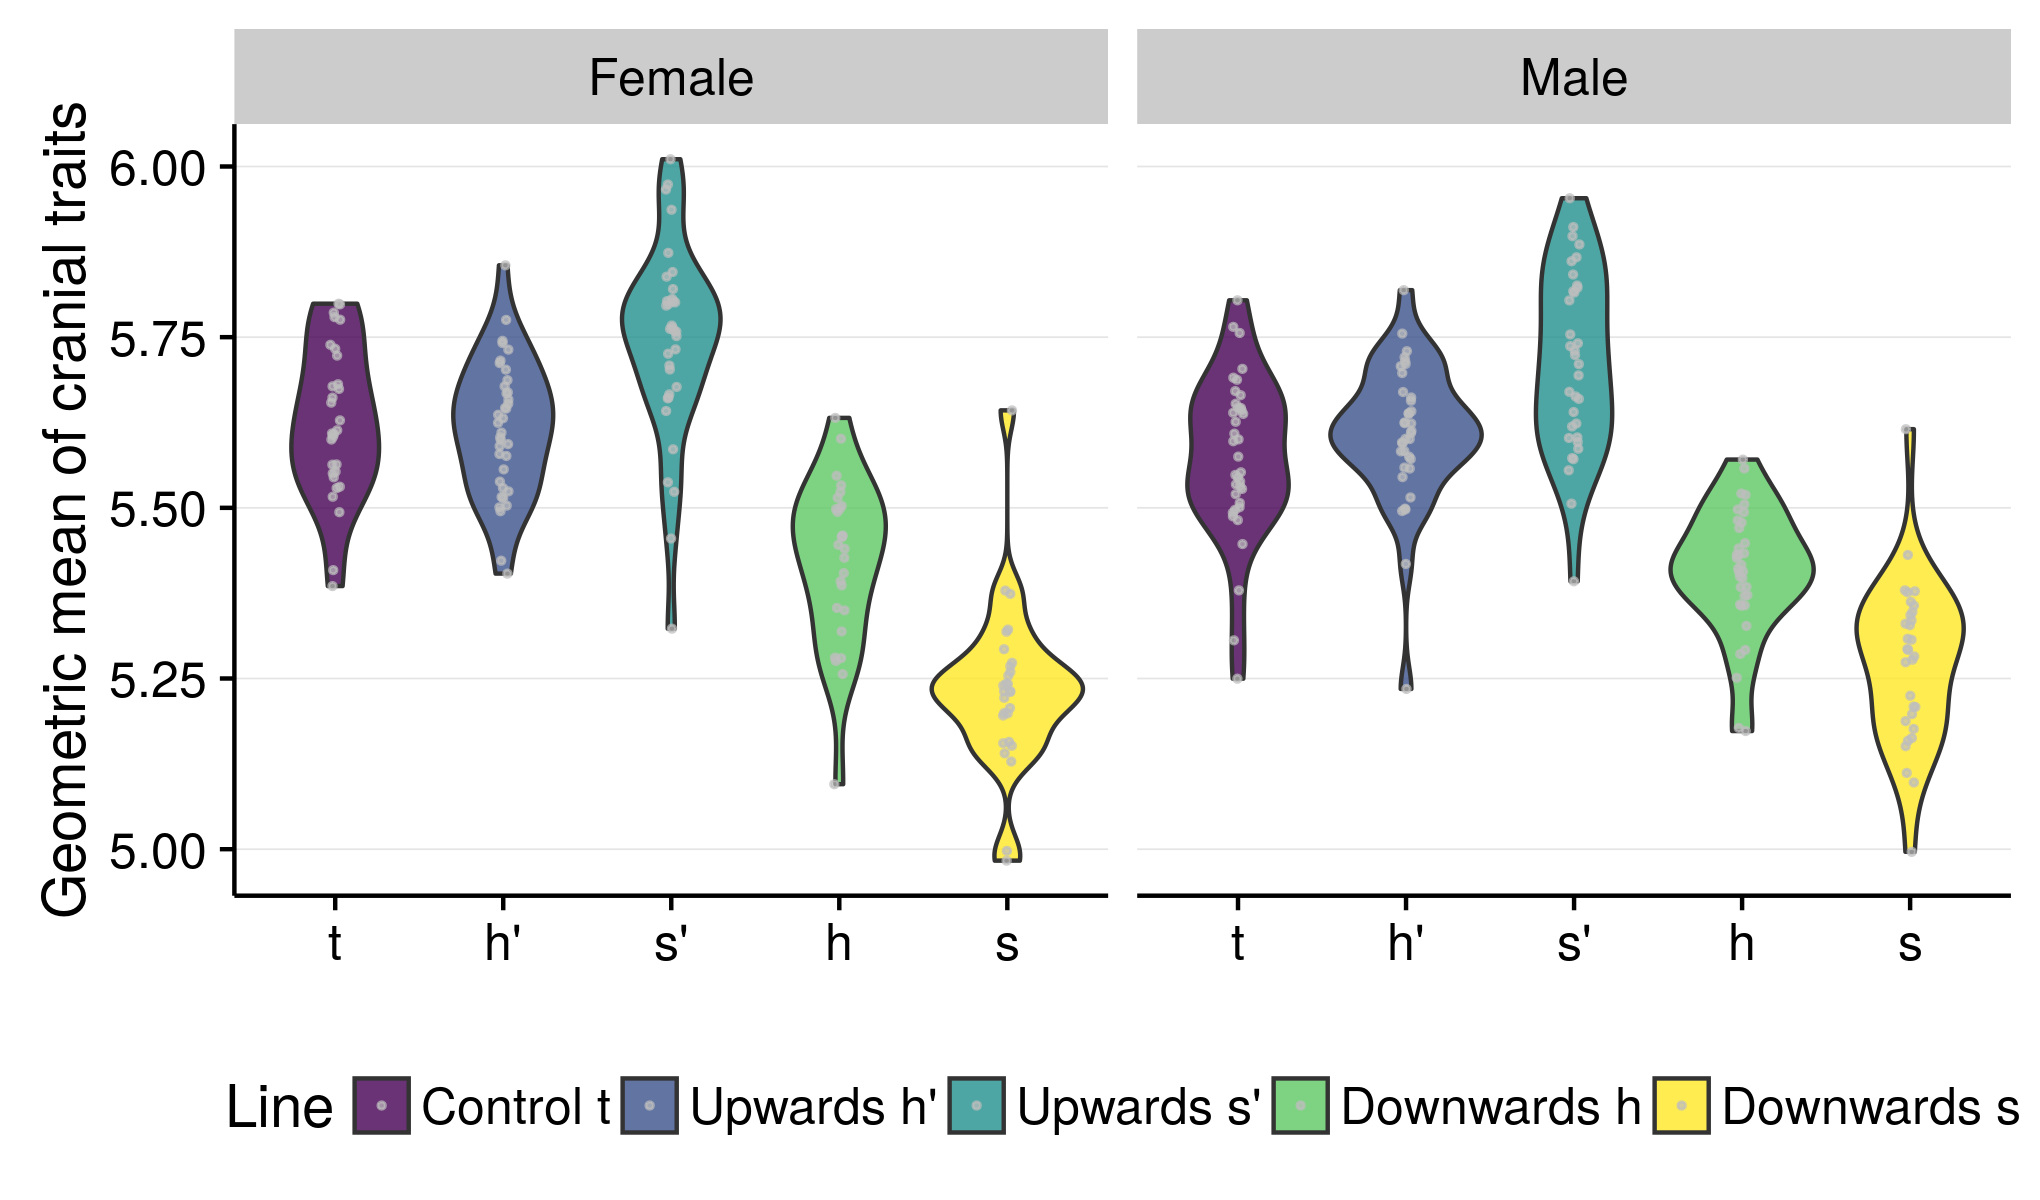
\includegraphics[width=\textwidth]{chapter_ratones/media/figure1.png}
    \caption[Selection response in weight]{Distribution of the
standardized isometric cranial size variable, calculated as the
geometric mean of cranial traits by line and gender. Upwards lines are
larger than downwards lines, while control line t is similar to the
upwards lines.}
    \label{fig-gmchange}
\end{figure}


\subsection{Matrix comparisons}


In the Krzanowski subspace comparisons all eigenvalues were not
significantly different between the observed and randomized matrix
comparisons (Fig. \ref{fig-comparisons}A). As for the the Bayesian
Random Skewers projection, we identified several directions with
different amounts of phenotypic variation in each line (first few
directions in Fig. \ref{fig-comparisons}B and full results in Fig.
S7). In most directions, the control line has significantly more
variation than the selected lines. But this reduction is not uniform in
all directions, and in several directions the selected lines have
variation that is comparable to the control line. We provide in the
supporting information the same set of results using G-matrices
(Fig.~S8). These results are considerably more noisy in several cases,
but consistent with the results obtained using the P-matrices.

\begin{figure}
    \centering
    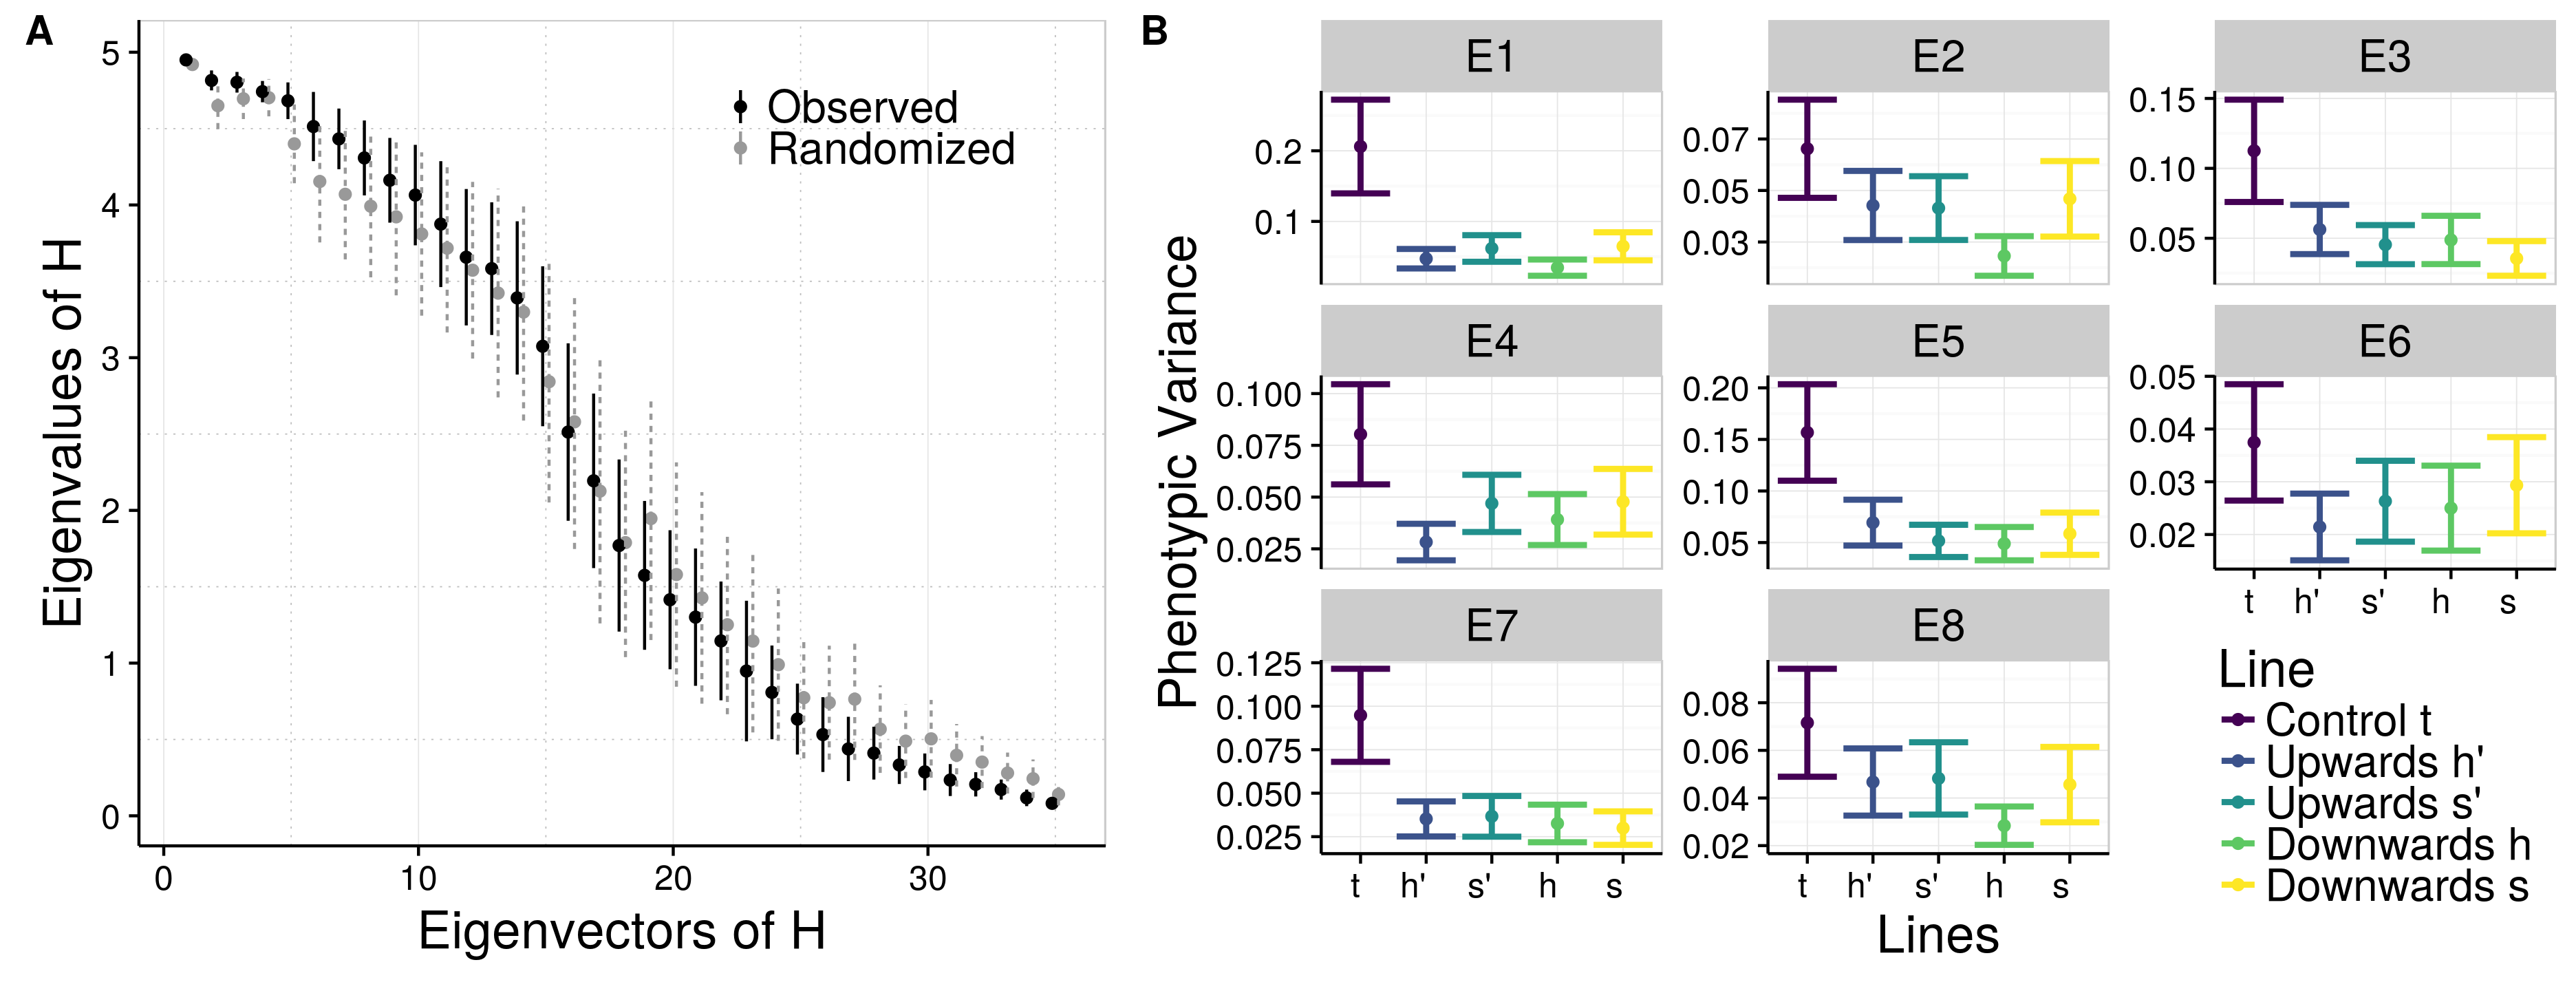
\includegraphics[width=\textwidth]{chapter_ratones/media/figure2.png}
    \caption[Matrix comparisons between selected and control lines]{(A) Bayesian Krzanowski
shared subspace. Eigenvalues for the H matrix are not significantly
different in the randomized and observed matrices, indicating a shared
subspace and a stable set of eigenvectors in all the lines. (B) Bayesian
Random Skewers Projection. Here we only show the first eight
eigenvectors of the decomposition, which are representative of the full
set of eigenvectors (Fig. S7). In most directions the control line has
higher variation than the selected lines, but in several directions the
control and selected lines show comparable levels of variation,
indicating that the loss of variation in the selected lines was not
uniform in all directions. A version of this figure using the G-matrices
is available in the Supporting Information (Fig. S8)}
    \label{fig-comparisons}
\end{figure}

\subsection{Evolutionary statistics}

The distribution of mean values of evolutionary statistics showed a rise
in integration and in the proportion of variation associated with the
first eigenvector when compared to the control t line (Fig.
\ref{fig-stats}A and B). All selected lines also showed a decline in
evolvability and flexibility when compared to the control (Fig.
\ref{fig-stats}C and D). First eigenvectors for each line are given in
table~S4, along with correlations between the first eigenvector and an
isometric size vector. All correlations between E1s and the isometric
vector were higher than \(0.71\), indicating that all first eigenvectors
are related with cranial size.

\begin{figure}     
	\centering
	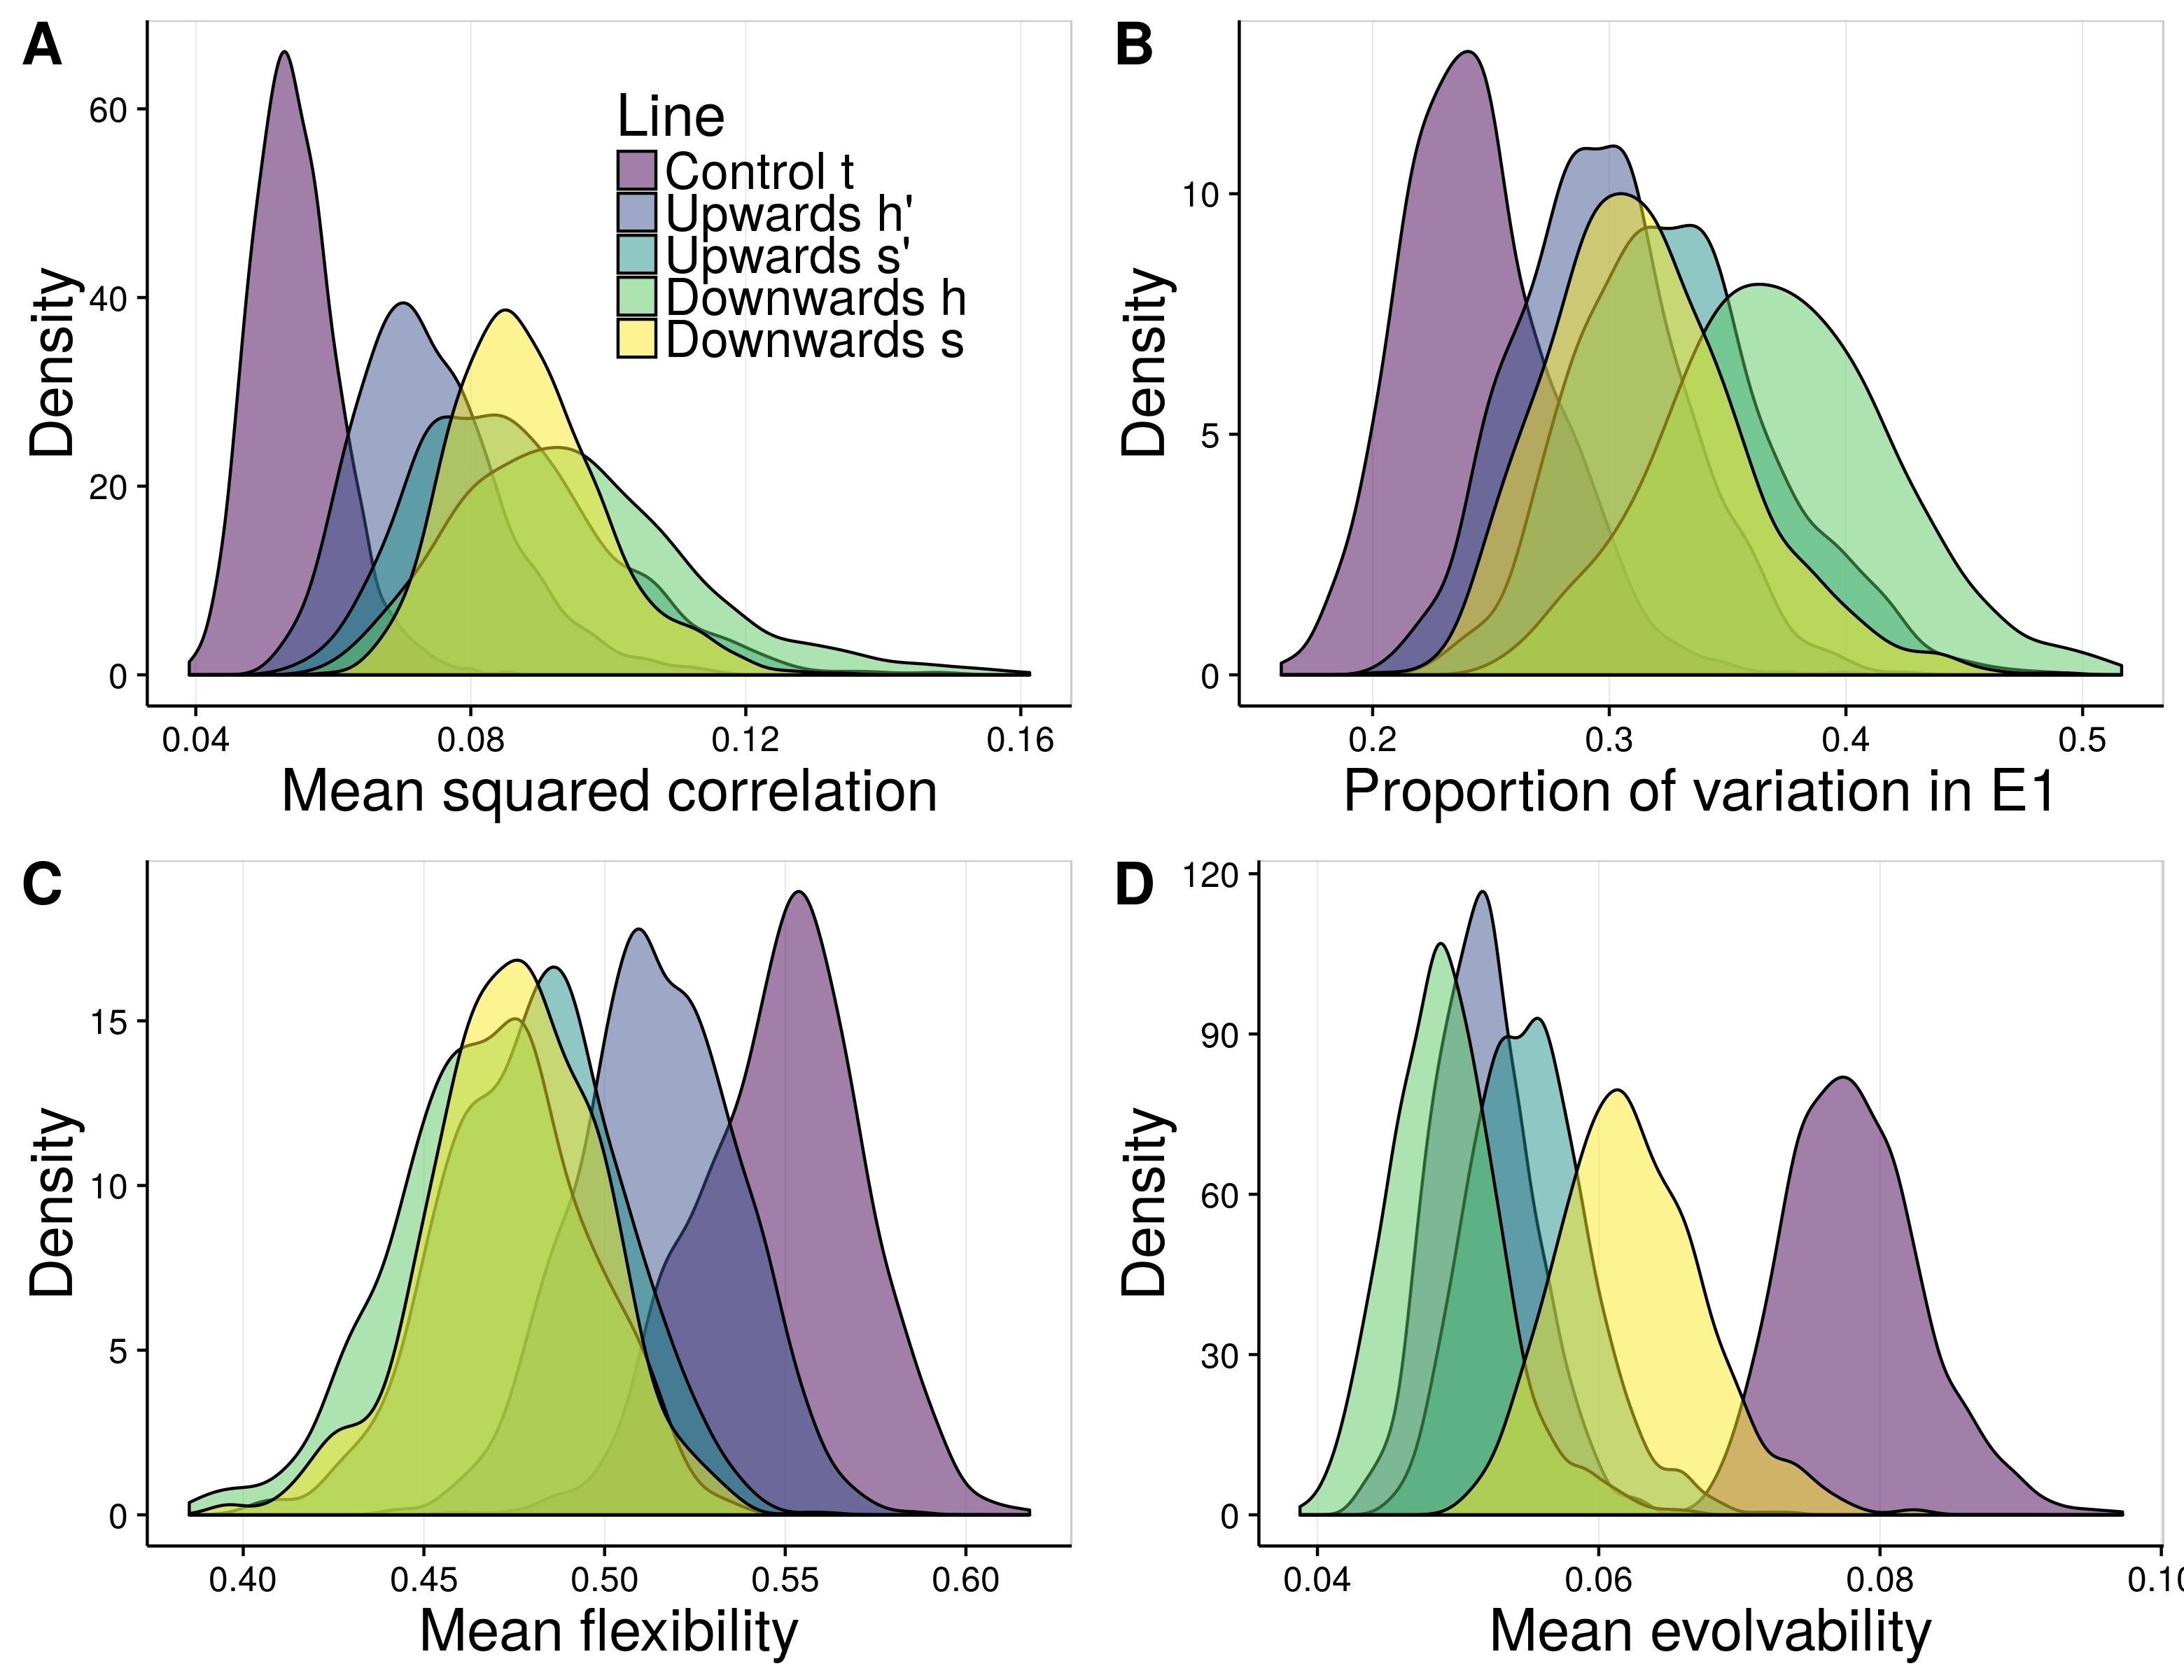
\includegraphics[width=\linewidth]{chapter_ratones/media/figure3.png}
	\caption[Evolutionary statistics in selected and control lines]{     Comparison
of covariation patterns between control and selected lines using evolutionary
statistics (A) Magnitude of integration measured as mean squared correlation
between all traits; (B) Proportion of variation associated with the first
eigenvector, which is related to size variation; (C) Mean flexibility; (D) Mean
evolvability. Curves represent posterior distributions obtained using the sample
of P-matrices from the BSFG model. Confidence interval and mean for all curves
can be found in Table S5. The same set of results using G-matrices are available
in Fig.~S9. G-matrix results are noisier, but consistent with the results
obtained using the P-matrices, suggesting the changes we observed indeed
occurred in the G-matrices.}     
	\label{fig-stats} 
\end{figure}

The scaled directional evolvability, the ratio of evolvability in the
direction of \(\delta z\) and the mean evolvability, shows a clear
increase with selection, with selected lines showing about double the
ratio observed in the control line (Fig. \ref{fig-dzpc1}A). The vector
correlation between \(\delta z\) and the E1 increased in all selected
lines, while this correlation in the control line shows a lower mean
correlation (around 0.6) and wider posterior distribution. Downward
selected lines have correlations of first eigenvector and \(\delta z\)
above 0.9 and upwards selected lines above 0.75 (Fig. \ref{fig-dzpc1}B).

\begin{figure}
    \centering
    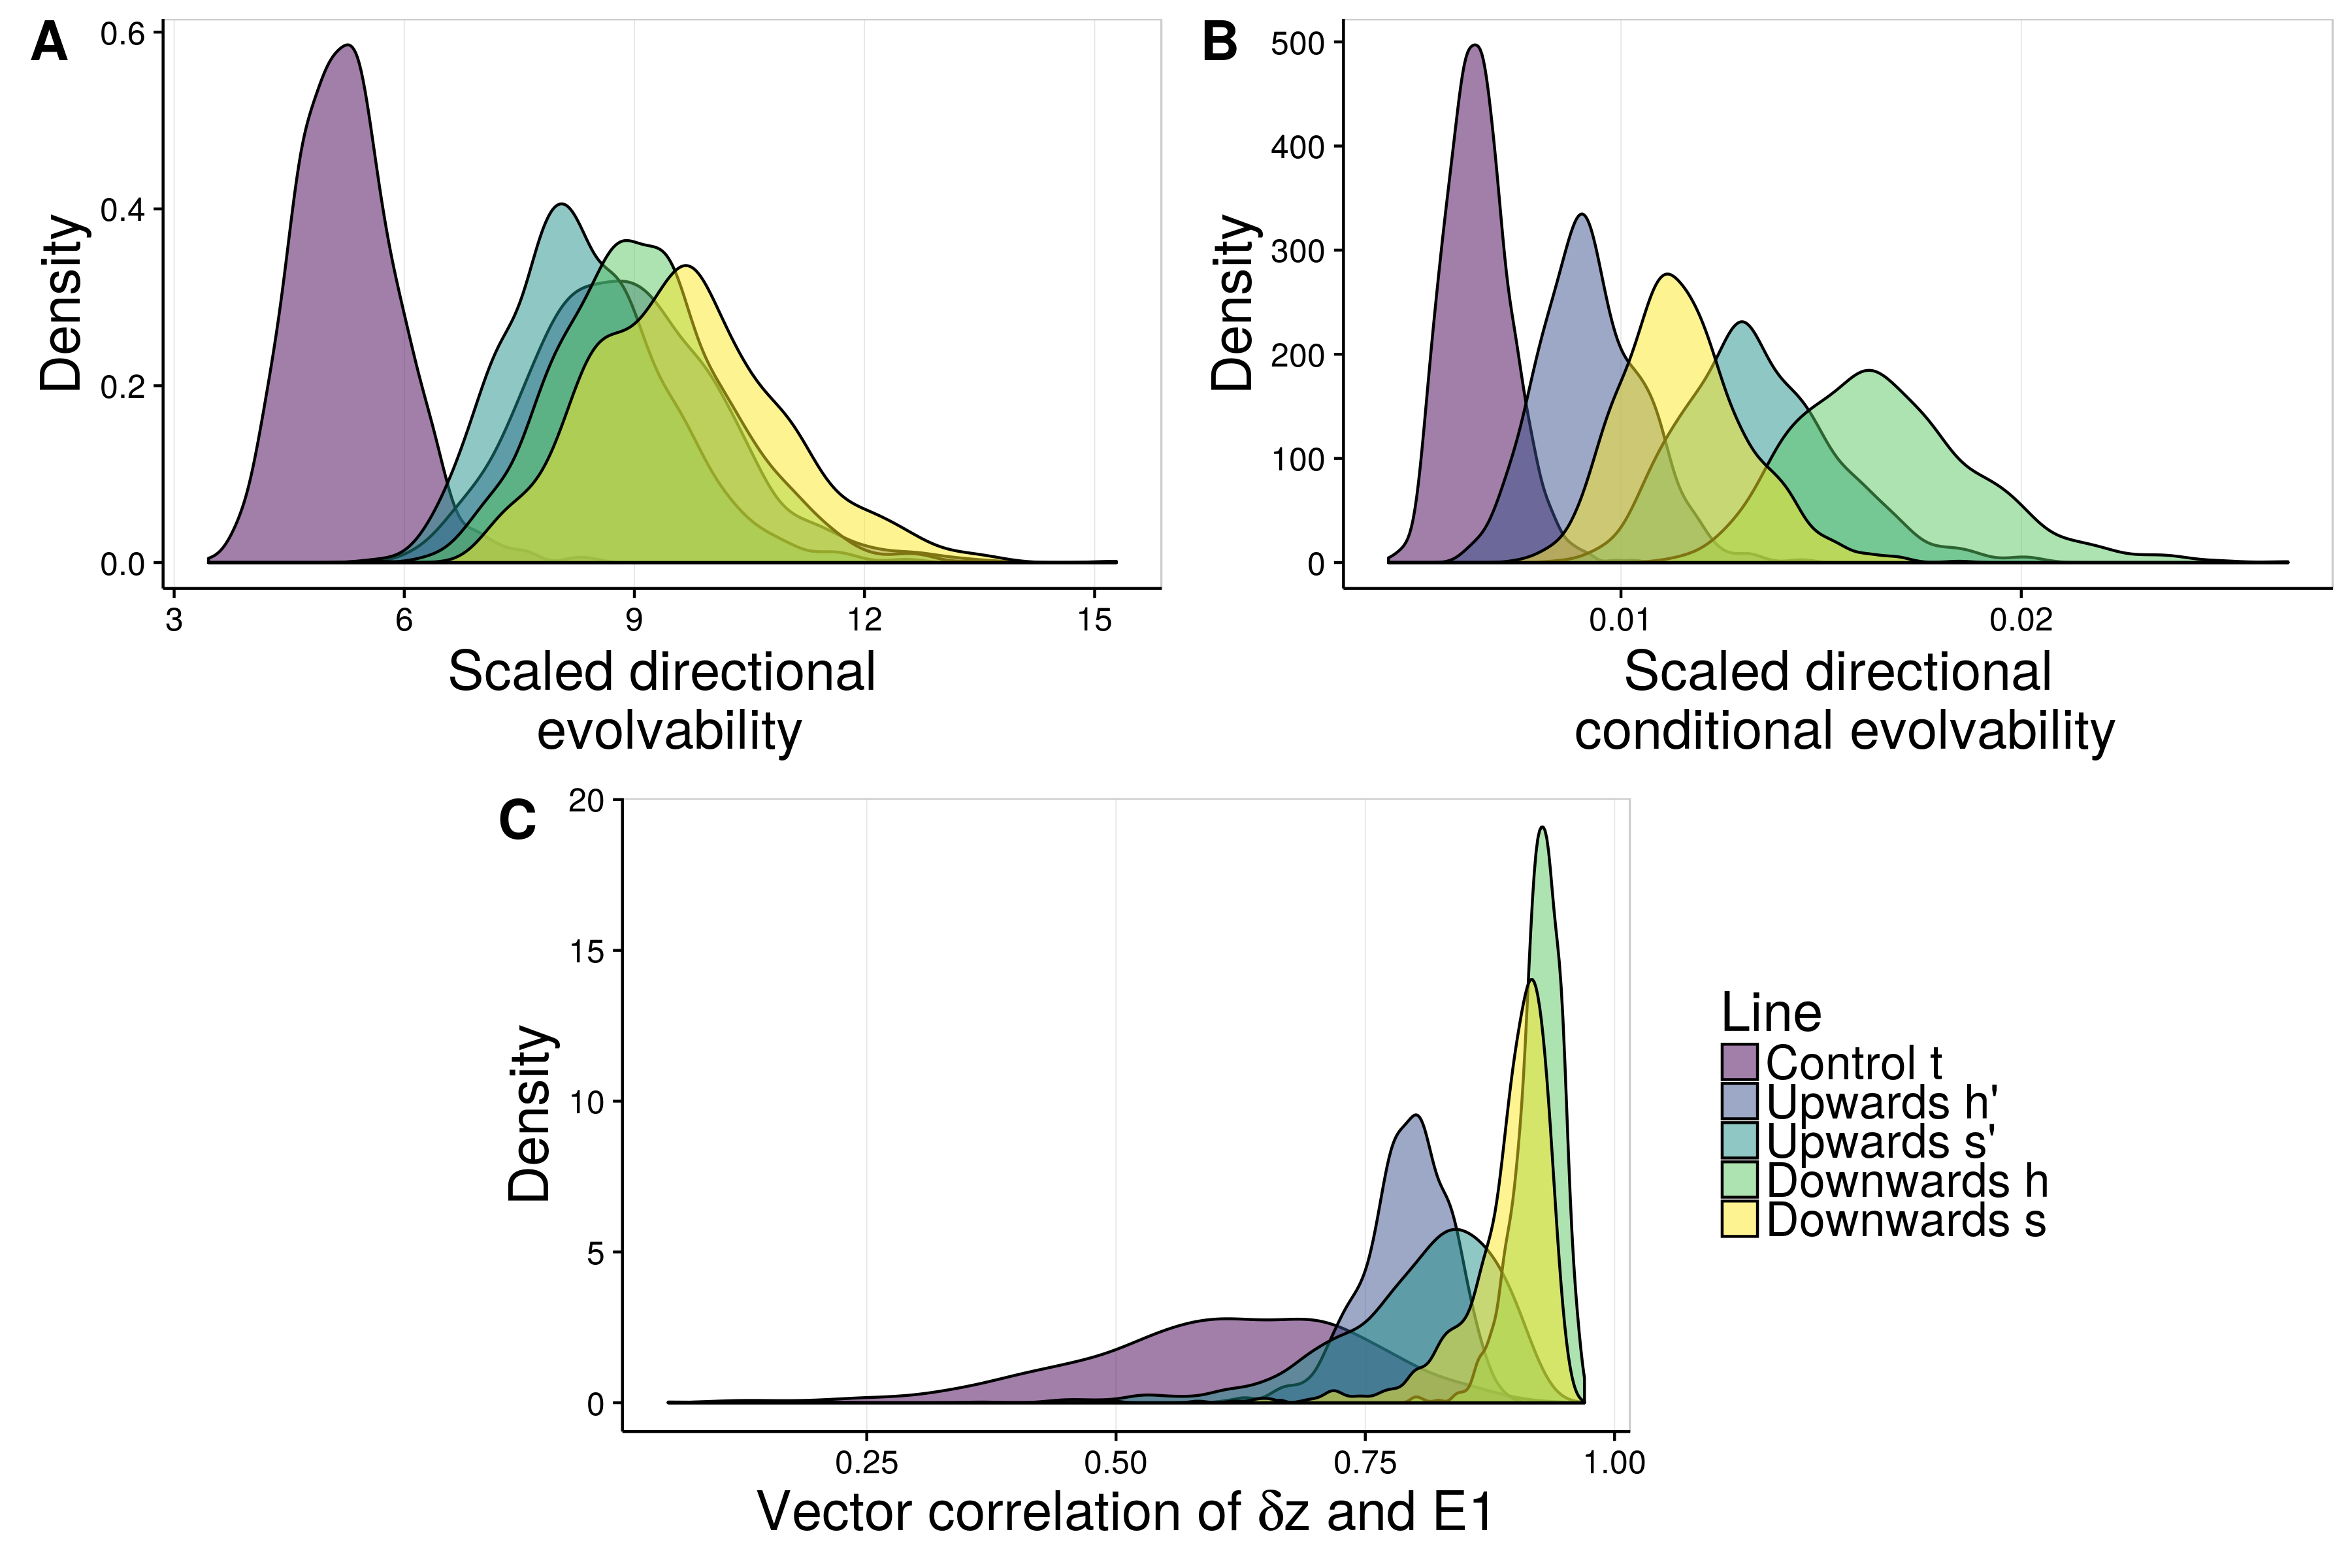
\includegraphics[width=\textwidth]{chapter_ratones/media/figure4.png}
    \caption[Directional evolutionary statistics in selected and control lines]{(A)
Scaled direction evolvability, the ratio of evolvability in the
direction of phenotypic divergence (\(\delta z\)) and the mean
evolvability for each line; (B) Scaled direction conditional
evolvability, the ratio of conditional evolvability in the direction of
\(\delta z\) and the mean conditional evolvability for each line; (C)
the vector correlation between \(\delta z\) and first eigenvector for
each line. Curves represent posterior distributions obtained using the
sample of P-matrices from the BSFG model. Confidence interval and mean
for all curves can be found in Table S6. The same set of results using
G-matrices are available in Fig.~S10. G-matrix results are noisier, but
consistent with the results obtained using the P-matrices, suggesting
the changes we observed indeed occurred in the G-matrices.}
    \label{fig-dzpc1}
\end{figure}

\section{Discussion}

Our experimental approach allows us to investigate how directional
selection alters multivariate covariation, and what are the consequences
of this interaction to evolution and diversification. Selected lines
diverged in both weight and cranial traits, and the changes in the
cranium were aligned with the main axis of variation, which is a
direction associated with cranial size. While to some extent this is an
unsurprising result given that selection was on overall size, our
results illustrate how rapidly covariation can change under directional
selection. In particular, the magnitude of association between traits is
more malleable than the pattern of association.

Patterns of covariation were fairly similar in all lines, a result
consistent with the observed pattern for natural populations of mammals
in general, even when comparing covariation between different
orders~\parencite{Porto2009-pi}. Krzanowski subspace comparison showed all the
lines share the subspace spanned by the first half of the eigenvectors.
Regarding the distribution of variation, the Bayesian Random Skewers
showed that in some directions the control line has more variation than
the selected lines, while in others control and selected lines have
comparable levels of variation. Taken together, these matrix comparison
results indicate a stable set of eigenvectors, spanning a similar space
in all the lines, and a non-isotropic reduction in variation in the
selected lines, that is, some directions lost more variation than others
(Figs. \ref{fig-comparisons} and S7).

As for integration, all selected lines increased their magnitude of
association between traits. The maximum observed difference in mean
squared correlation is almost 0.05 (when comparing the control t line
and the downwards h line) a difference comparable to those observed
between mammalian orders~\parencite{Marroig2009-gf}. This increase in
integration is mirrored by the observed increase in the proportion of
variation associated with the first eigenvector, which is related to
size. This is expected, because size variation can be interpreted as
coordinated variation in all traits, and so an increase in size
variation leads to higher correlations between all traits
\parencite{Porto2013-dc}. Therefore, the rise in integration in the selected
lines is due to an increase in the proportion of variation that is
related to cranial size (which changed due to selection on overall
size).

This increase in integration is also reflected in the flexibility, which
is lower in all the selected lines. Flexibility measures the ability of
a population to respond in the direction of selection, and because a
larger proportion of cranial variation in the selected lines is
concentrated in size variation, less variation is available to respond
in other directions. Also, the mean evolvability, or total available
variation for responding to selection, is smaller in the selected lines.

At first sight, this is compatible with the idea that directional
selection depletes variation. However, focusing only on the reduction of
total variation is misleading. Taking the multivariate aspect of this
system in consideration, the distribution of the available variation is
also changing. Although total variation in all directions is smaller in
the selected lines (Fig. \ref{fig-stats}, panel D), the increase in
the proportion of variation associated with the first eigenvector (Fig.
\ref{fig-stats}, panel B) (which is highly related to cranial size,
Table S4) means the proportion of variation in the direction of
evolutionary divergence is in fact increasing in the selected lines
(Fig. \ref{fig-stats}, panels A and B), and the first eigenvector is
also more aligned with the direction of divergence in the selected lines
(Fig. \ref{fig-dzpc1}C). This reorganization of variation is supported
by the change in the scaled directional evolvability and scaled
conditional evolvability, which show that the scaled variation in the
direction of divergence is almost doubled in selected lines when
compared to the control (Fig. \ref{fig-dzpc1}A and B).

This relative increase in variation is incompatible with the traditional
view of depletion of variation in the direction of selection due to the
fixation of additive alleles. Under a purely additive model of cranial
variation, as rare additive alleles with effects on size move to
fixation, they could increase genetic variation for size in the process
\parencite{Burger1995-qd}. In large populations this increase in variation under
directional selection can be maintained by new mutations that arise and
sweep to fixation. In principle we can't rule out this possibility, but
we are observing this effect after about 50 generations of strong
directional selection (Table~S1), after which we would expect the
initial increase of variation to have disappeared as those initially
rare alleles become fixed, and, because of our low effective population
sizes, the influx of new mutations should be negligible. Also, increase
in size variation due to additive alleles would be more likely to occur
in traits that are controlled by a small number of loci \parencite{Burger1995-qd, Jain2015-fj}, which is not likely to be the case for the cranium
\parencite{Leamy1999-dm, Wolf2005-nr, Porto2016-qc}. Furthermore, the genetic basis of
morphological covariation is unlikely to be purely additive
\parencite{Phillips2001-xb, Whitlock2002-yb}. The changes are also not likely to be
due to drift alone, as all the selected lines are consistent in their
covariation patterns, and under drift we would expect a more random
distribution of differences between the lines. However, epistatic
interactions can provide a source of standing variation that allows the
increase of variation in the direction of selection
\parencite{Cheverud1995-nm, Wagner2007-cx, Pavlicev2011-xm, Melo2015-bk}, and can bias
further mutations to be aligned with this direction
\parencite{Jones2007-xe, Jones2014-wj}.

Because genetic architectures can interact with selection in different
ways, we expect different outcomes depending on the complexity of the
genetic architecture underlying the set of traits under investigation:
additive variation is expected to be consumed in the direction of
selection, while epistatic variation can lead to an increase in
variation in the direction of selection.~\textcite{Careau2015-sy} showed that
directional selection on behavior traits follows the expectation of the
additive model, with a loss of variation in the direction of selection
and a plateau in the response to selection after a few generations. In
our experiment, as expected by the additive model, we also see a loss of
total variation in the selected lines, but this reduction is
non-isotropic. Some directions lost more variation than others, and the
direction of selection ended up with proportionally more variation in
the selected lines, suggesting the influence of epistasis and a more
complex genetic architecture underlying the covariation of cranial
traits.~\textcite{Assis2016-vz} reported the same kind of realignment of variation
and selection as we did, but saw no loss of variation in samples from
modern populations after selection, when compared to historical samples.
This could be related to the large effective sample sizes in the wild
chipmunk populations considered, and suggests that large populations can
reorganize covariation patterns in response to selection with no loss in
total variation. Neither our results nor those from~\textcite{Assis2016-vz} allow us
to evaluate limits in the response to selection in the cranium, leading
to plateaus in response, but we speculate that in large populations the
availability of standing epistatic variation and the biasing of new
mutations in the direction of selection could delay the onset of the
kind of plateau in multivariate evolutionary response seen
in~\textcite{Careau2015-sy}.

The observed increase in integration over a microevolutionary time scale
also has consequences for our understanding of macroevolutionary
patterns. In mammals, changes in the magnitude of integration are much
more common than changes in the pattern of trait association
\parencite{Porto2009-pi}. Our results suggest that these difference can be
explained by the pervasiveness of selection on size along the mammalian
clade \parencite{Marroig2005-ce, Baker2015-ti}. Lineages that underwent selection
on size might have higher integration, and those whose selective
response were not size-related might have lower integration. Also,
divergence that is aligned with covariation can not be interpreted as
only a product of constraints, since selection can directly reshape
variation \parencite{Punzalan2016-lb}.

Here we attempt to elucidate the effect of directional selection on
covariation, and how this impacts evolution. We use experimental
selection on size to answer this question, and find that selection can
actively restructure covariation, and, in addition of depleting
multivariate covariation, can reorganize standing covariation in the
direction of evolutionary response, increasing a population's relative
ability to respond to selection in that direction. This is in accordance
with recent models of phenotypic covariation that include a more
realistic genetic architecture, and an experimental evidence of
directional selection shaping variation in non-intuitive ways. Along
with recent empirical, theoretical, and simulation work, our results
reinforce a shift in our understanding of how populations are shaped by
natural selection. An obvious next step is to combine this sort of
experimental selection with genetic mapping to understand, at the
genomic level, how this reorganization of variation is taking place.

\section*{Acknowledgments}\label{acknowledgments}

Andrea Kaufmann-Zeh helped with the initial draft of this manuscript.
Harley Sebastião and Barbara Costa helped with data acquisition. Julia
Laterza Barbosa made the cranium illustrations showing the landmarks.
Monique Simon, Guilherme Garcia, Fabio Machado, Jason Wolf, Michael
Turelli and Günter Wagner provided helpful comments and discussion on
the manuscript. Comments by Luis-Miguel Chevin, Mihaela Pavlicev and one
anonymous reviewer helped improve the final version of this manuscript.

AP is funded by FAPESP grant number 2013/06577-8, DM is funded by FAPESP
grant number 2014/26262-4, GM is funded by FAPESP grant number
2011/14295-7.

\section*{Author Contributions}

GM and MO designed the research. MO and SB conducted the selection
experiments. AP cleaned and measured all animals. AP, DM and GM designed
the analysis. AP and DM performed the analysis and wrote the initial
draft. AP, DM, MO and GM reviewed and edited the final manuscript.

\printbibliography

\section*{Supporting Information} % (fold)

\makeatletter
\renewcommand{\thefigure}{S\arabic{chapter}.\arabic{figure}}
\makeatother

\makeatletter
\renewcommand{\thetable}{S\@arabic\c@table}
\makeatother

\setcounter{figure}{0}
\setcounter{table}{0}

\begin{figure}
    \centering
    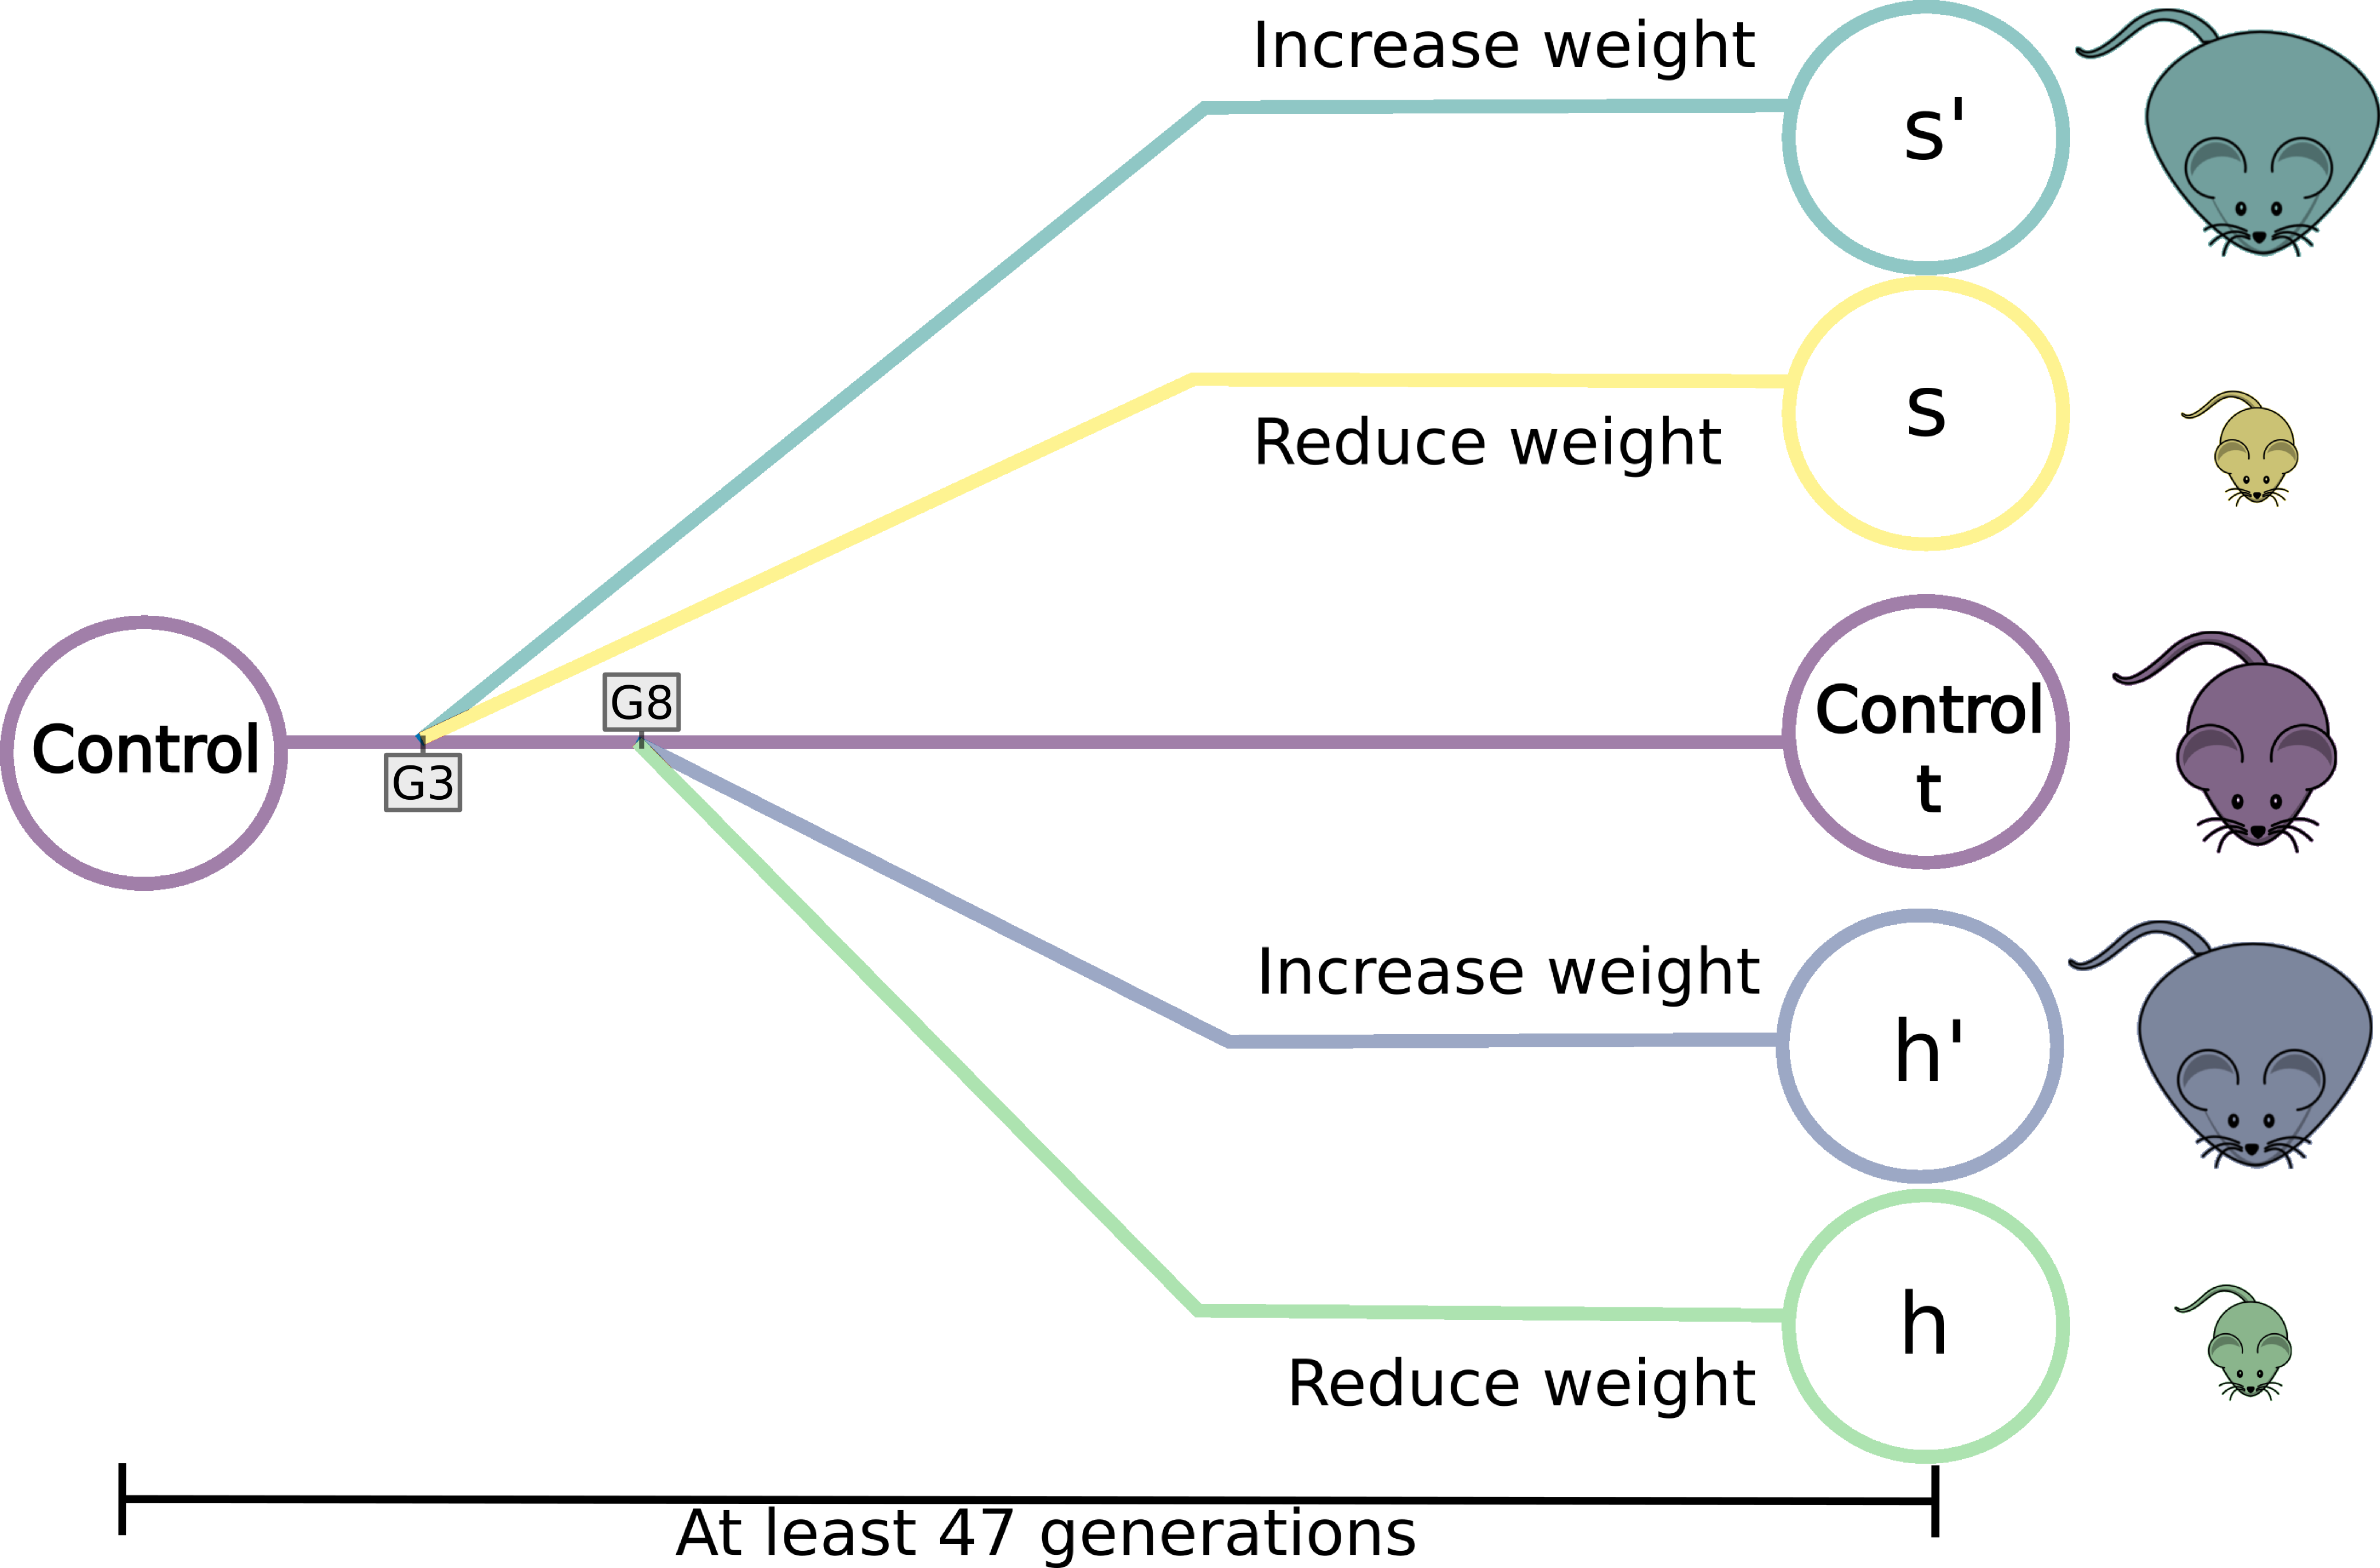
\includegraphics[width=12cm]{chapter_ratones/media/SI/figureS1.png}
    \caption[Experimental scheme]{Scheme of relationship between mice lines used in the study. Selection regime for body weight at 49 days was conducted in s and h lines for reduction, in s' and h' lines for increase, and a control line was maintained with random mating along generations, but avoiding full-sib matings. In downwards s and upwards s' lines inbreeding was performed by limiting population size and in downwards h and upwards h' full-sib mating was performed only during first generations.}
    \label{figsup:experiment}
\end{figure}

\begin{table}
\centering
\caption[Sample sizes per generation]{Number of animals per generation, inbreeding coefficients and selection differentials by line.
N average number of weighted individuals per generation. Ne effective population size. \%d percentage of animals that left descendants. $F_{50}$ increase in inbreeding coefficients for each line since the foundation, calculated as $F_{G}=\frac{1}{2N} + (1-\frac{1}{2N})F_{G-1}$.
Standard cumulative selection differential (SD) at $50^{th}$ generation per sex for each line, calculated as the sum of selection differential over 50 generations divided by the standard deviation.
}
\vspace{0.2cm}
\begin{tabular}{rlccccccc}
  \hline
		Selection & Line &  N  & Ne & \%d &  $F_{50}$ & $SD_{females}$ & $SD_{males}$ \\
  \hline
		Control   & t    & 162 & 40 & 24 & 0.48 &   2.5 &   6.9 \\
 		Downwards & h    &  59 & 12 & 16 & 0.91 & -15.1 & -23.1 \\
 		Downwards & s    &  59 &  8 & 20 & 0.91 & -24.3 & -25.6 \\
 		Upwards   & h'   &  69 & 12 & 12 & 0.93 &  43.3 &  47.0 \\
 		Upwards   & s'   &  74 &  8 & 14 & 0.93 &  45.8 &  46.8 \\
   \hline
\end{tabular}
\end{table}\label{table:linesdetailed}

\begin{table}
\centering
\caption{Sample sizes by line and sex.}
\begin{tabular}{rlcccc}
  \hline
Selection     & Line  & Generations           & Females & Males & Total \\
  \hline
    Control   & t     & $55^{th}$             &  30 &  37 &  67 \\
	Downwards & h     & $47^{th}$, $48^{th}$ &  27 &  35 &  62 \\
	Downwards & s     & $52^{th}$, $53^{th}$ &  28 &  31 &  59 \\
	Upwards   & h'    & $47^{th}$             &  37 &  36 &  73 \\
	Upwards   & s'    & $52^{th}$             &  34 &  34 &  68 \\

   \hline
\end{tabular}
\end{table} \label{table:samplesizes}

\begin{figure}
\centering
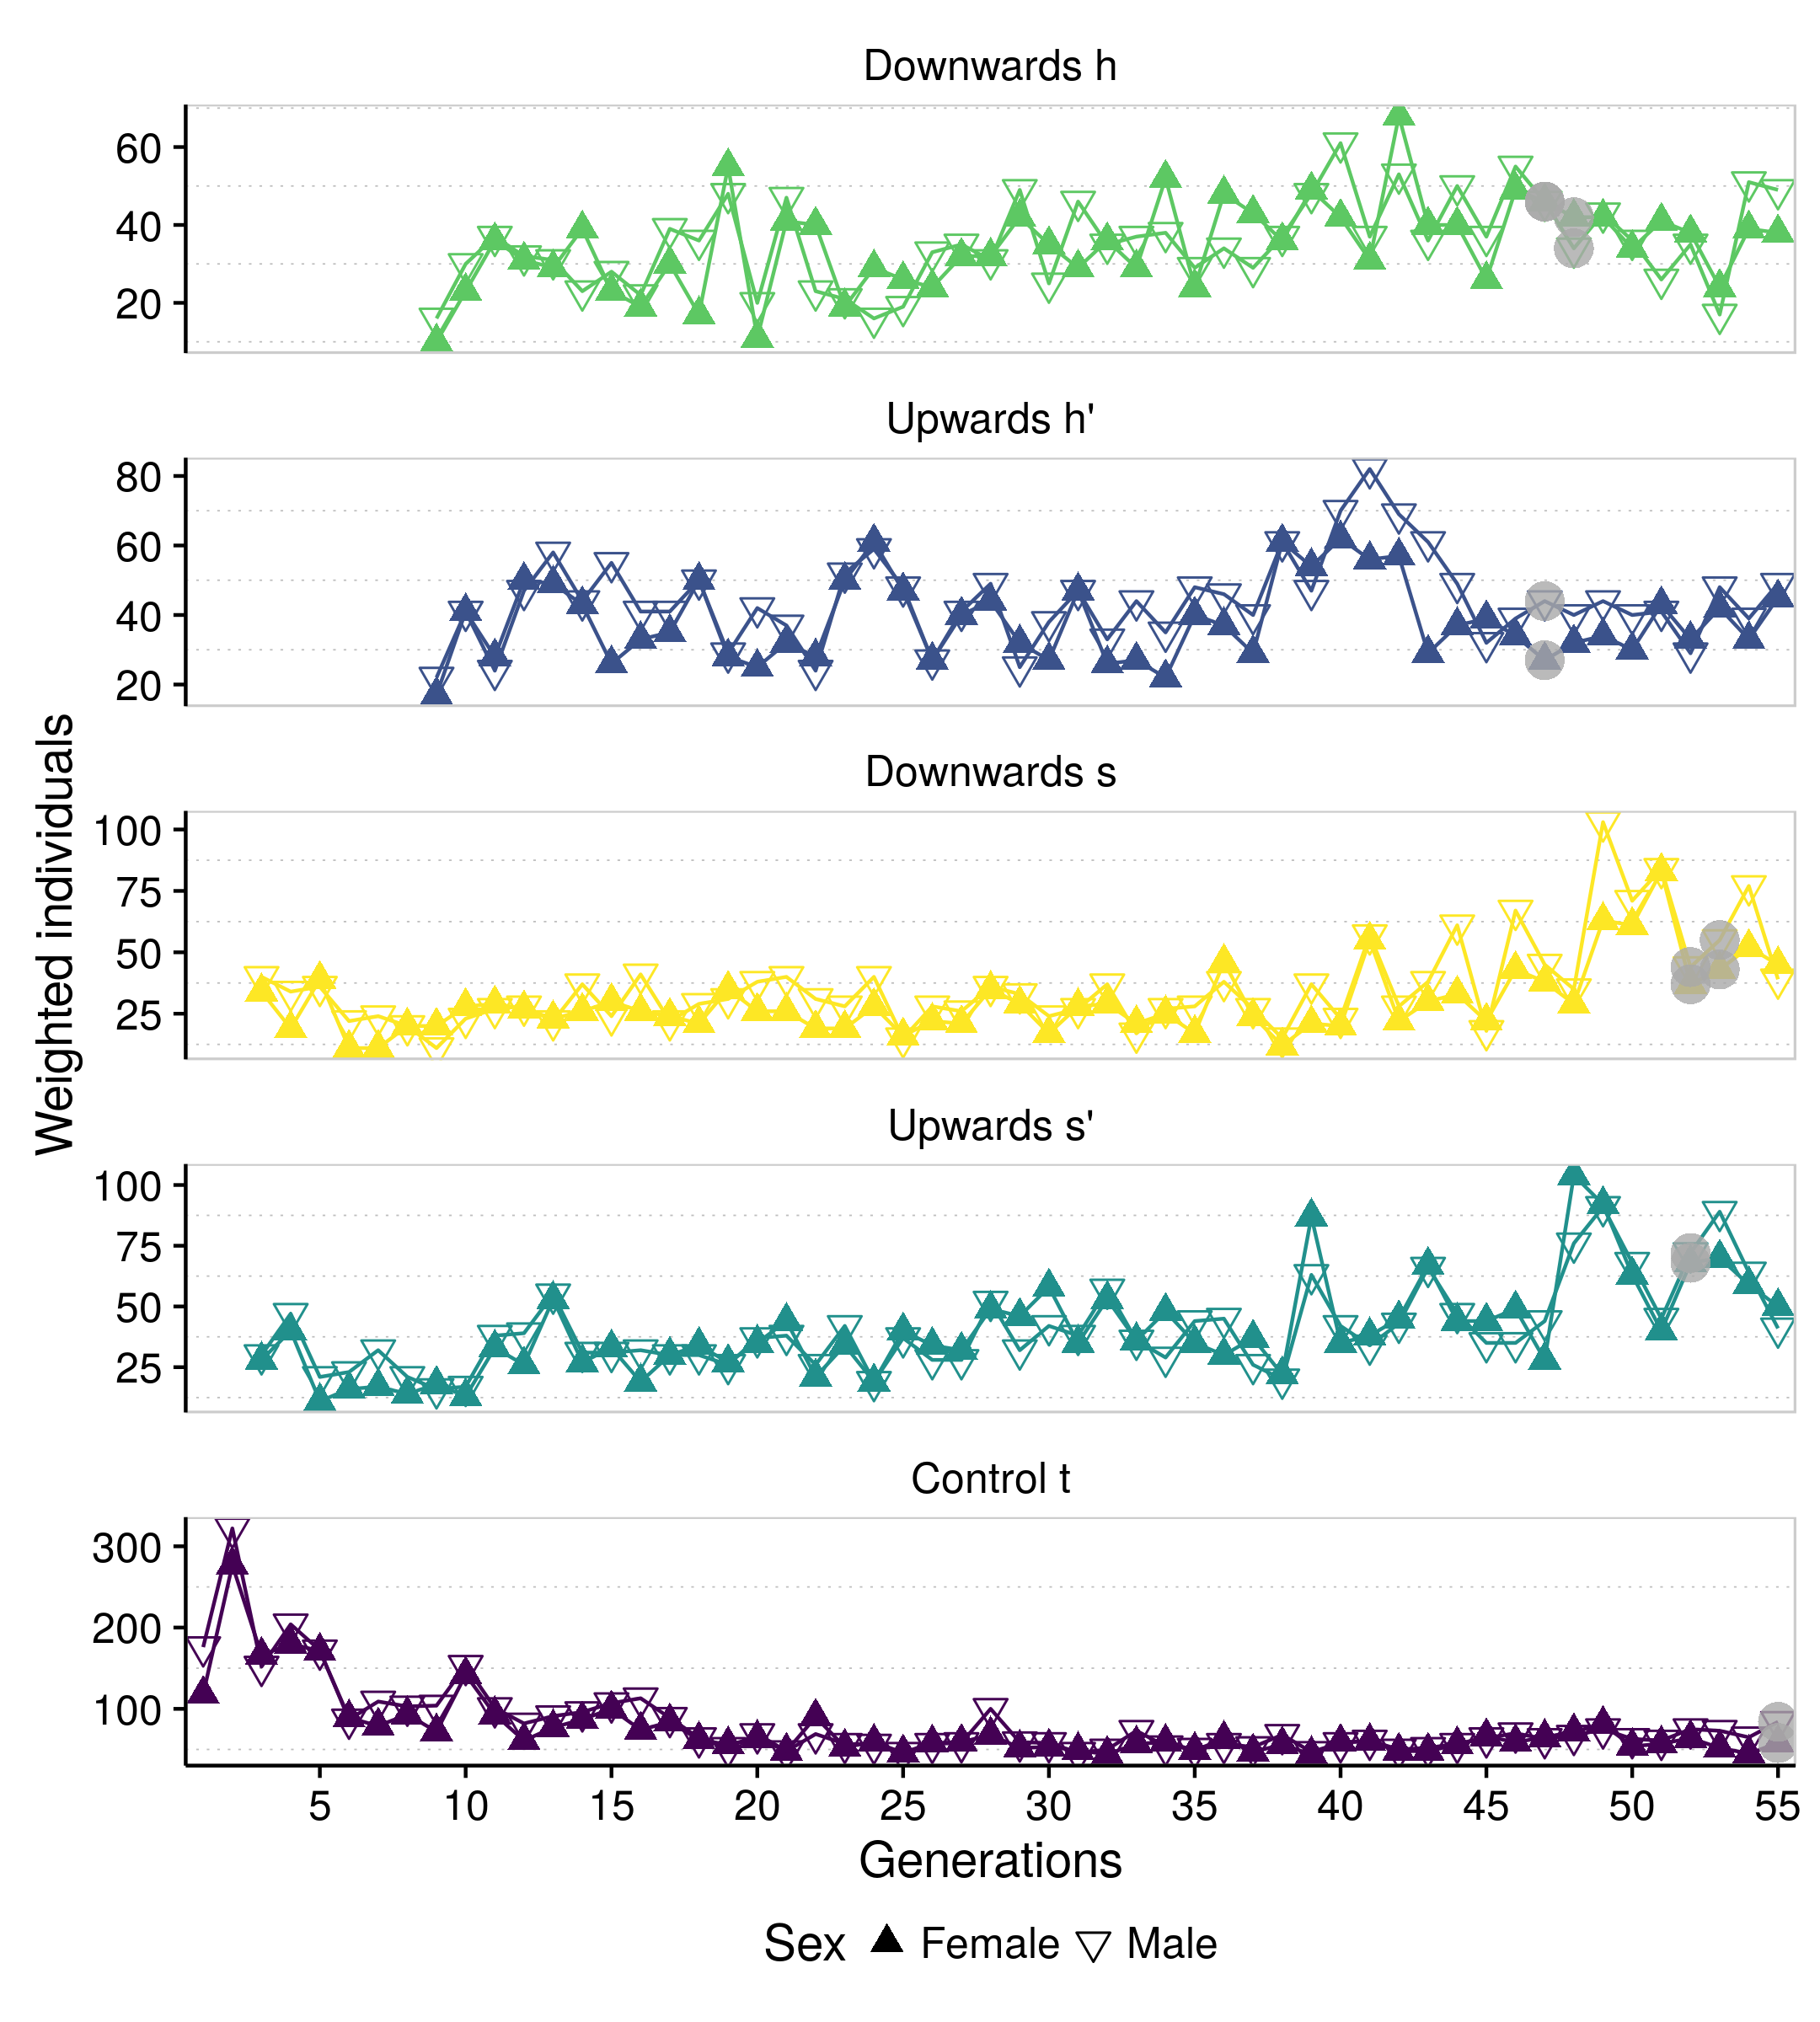
\includegraphics[width = 12cm]{chapter_ratones/media/SI/figureS2.png}
\caption[Samples per generation]{Number of weighted animals per generation by line and sex. Grey circles highlight the generations used in this study.}
\end{figure}

\begin{figure}
\centering
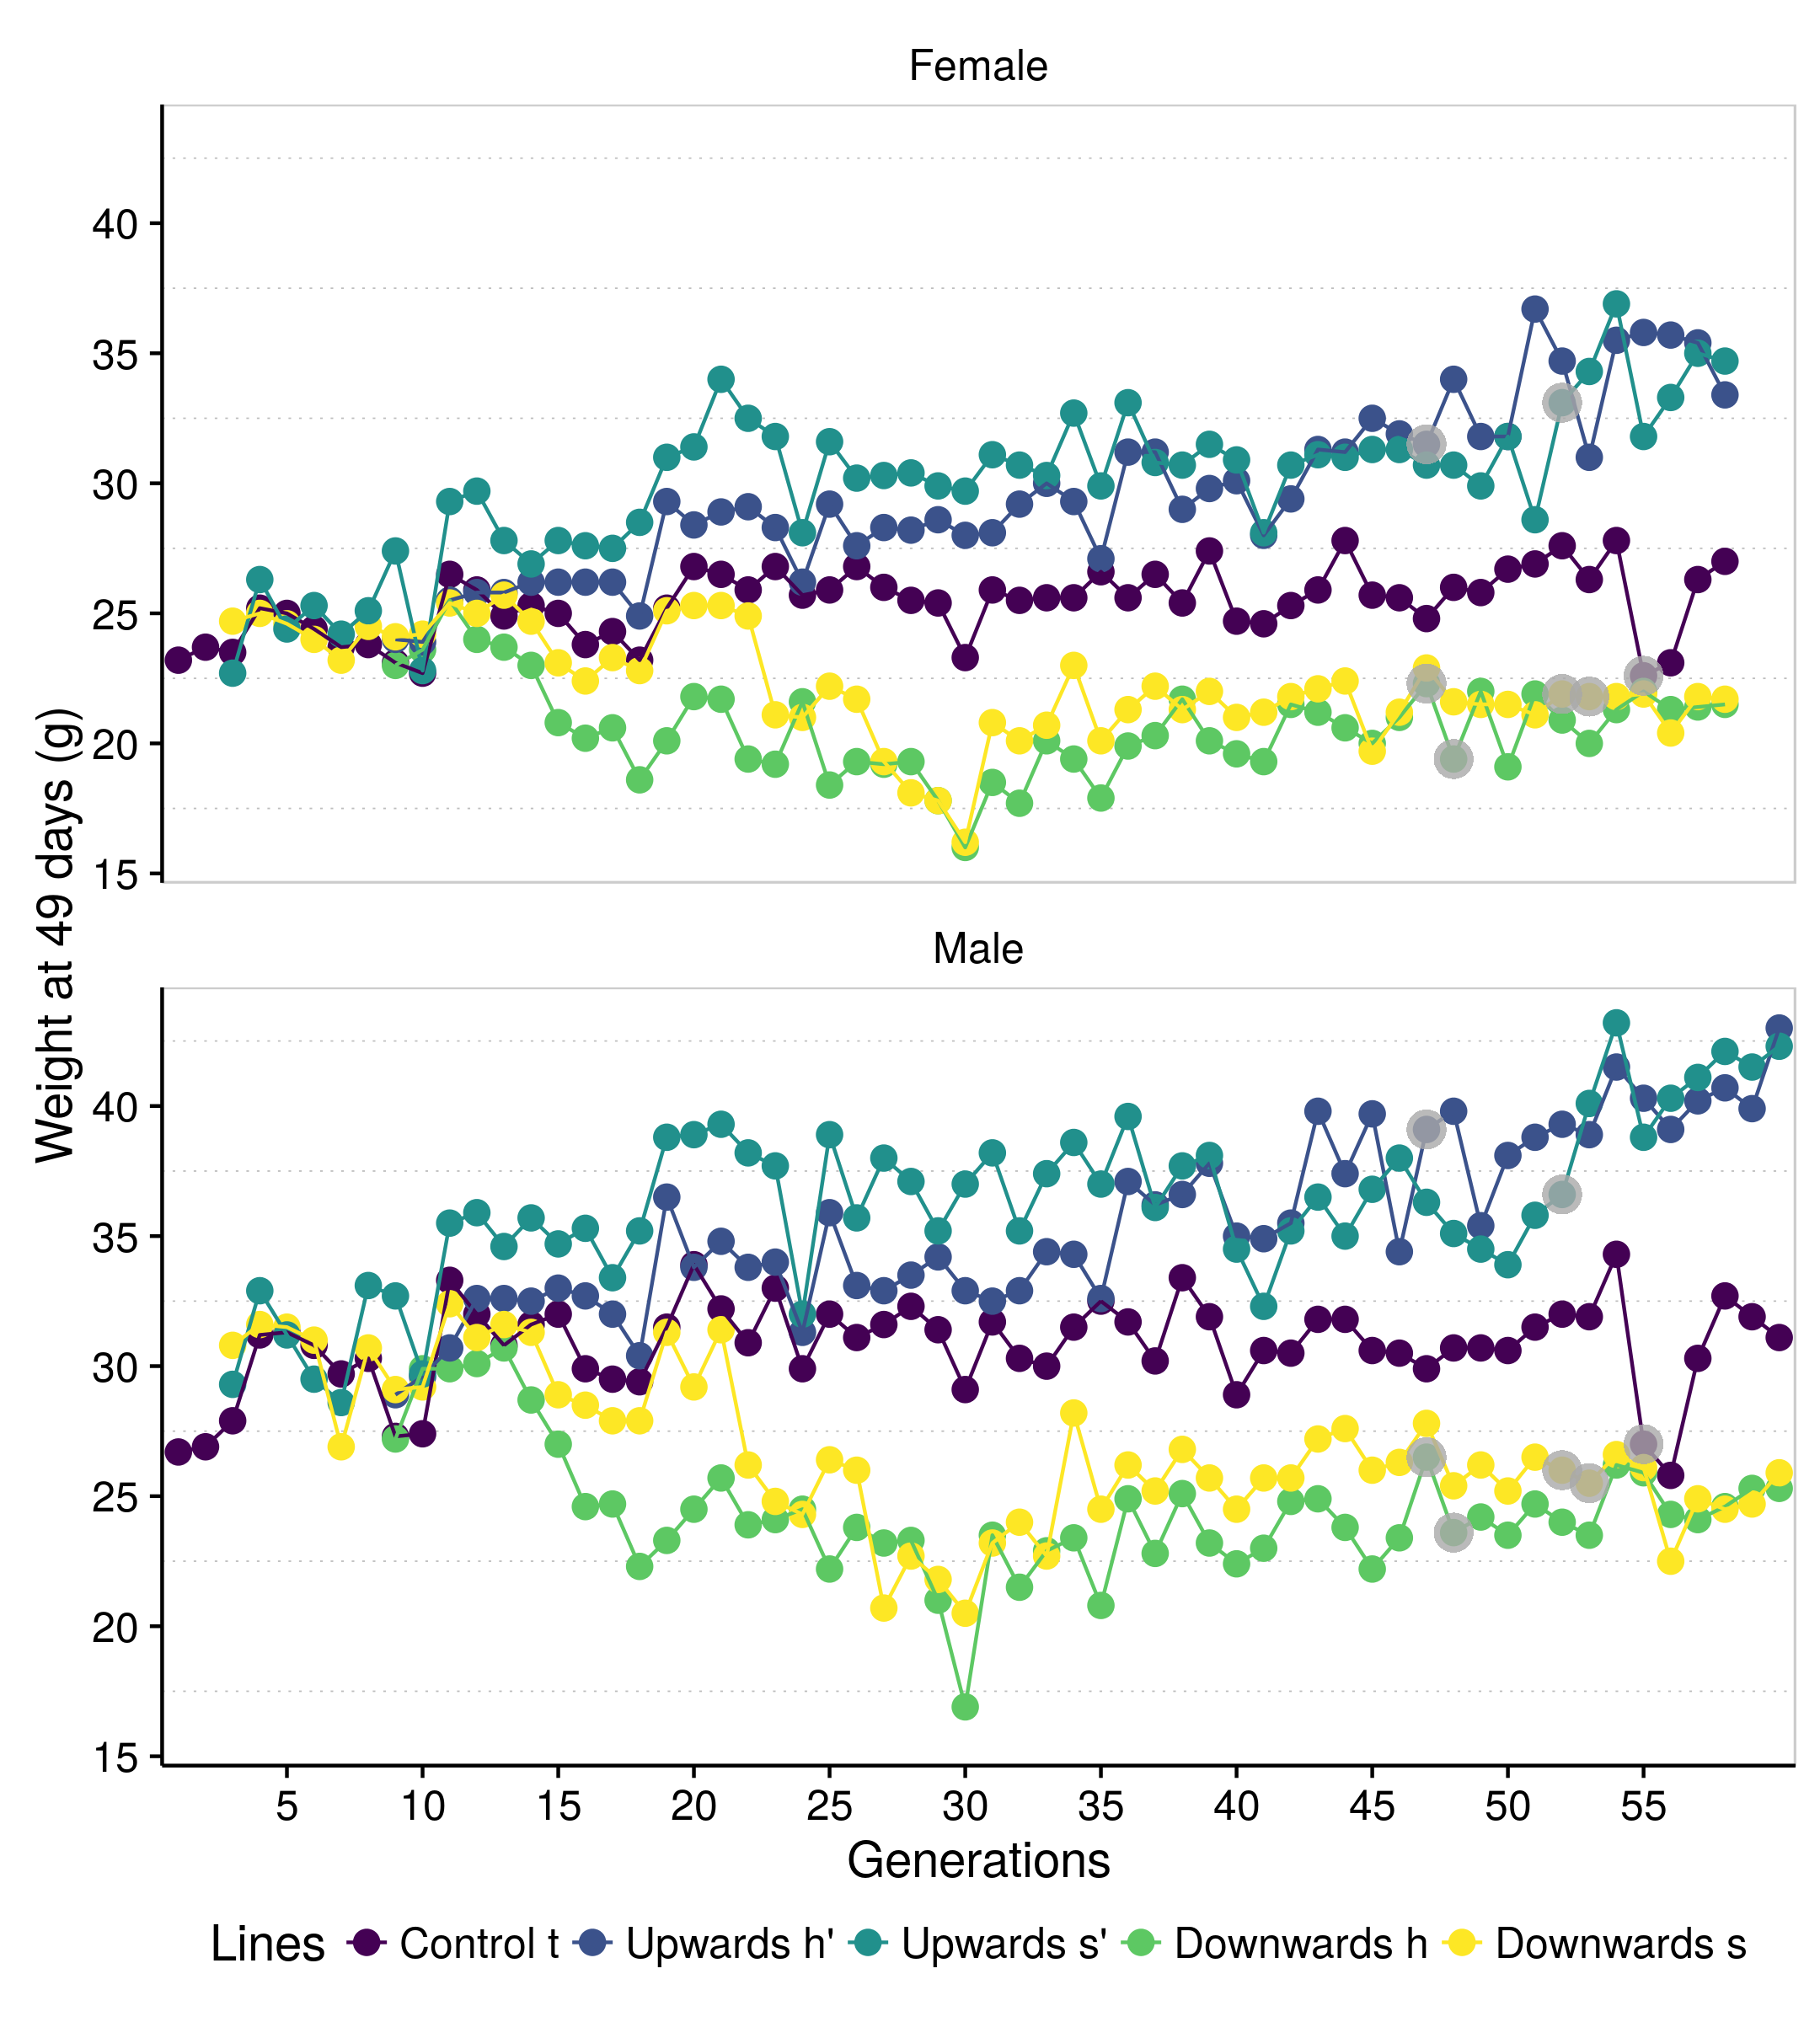
\includegraphics[width = 12cm]{chapter_ratones/media/SI/figureS3.png}
\caption[Evolution of body weight]{Average weight at 49 days per generation by line and sex, for the full experiment. Grey circles highlight the generations used in this study. We can see that after around the first 15 generations, besides some fluctuations, all selected lines consistently responded to directional selection, being the upward selected line heavier than control t line and downward selected lines lighter than the control t line. After the 56th generation, the mean weight of control t line was similar to that of the previous generations.}
\end{figure}

\begin{figure}
    \centering
    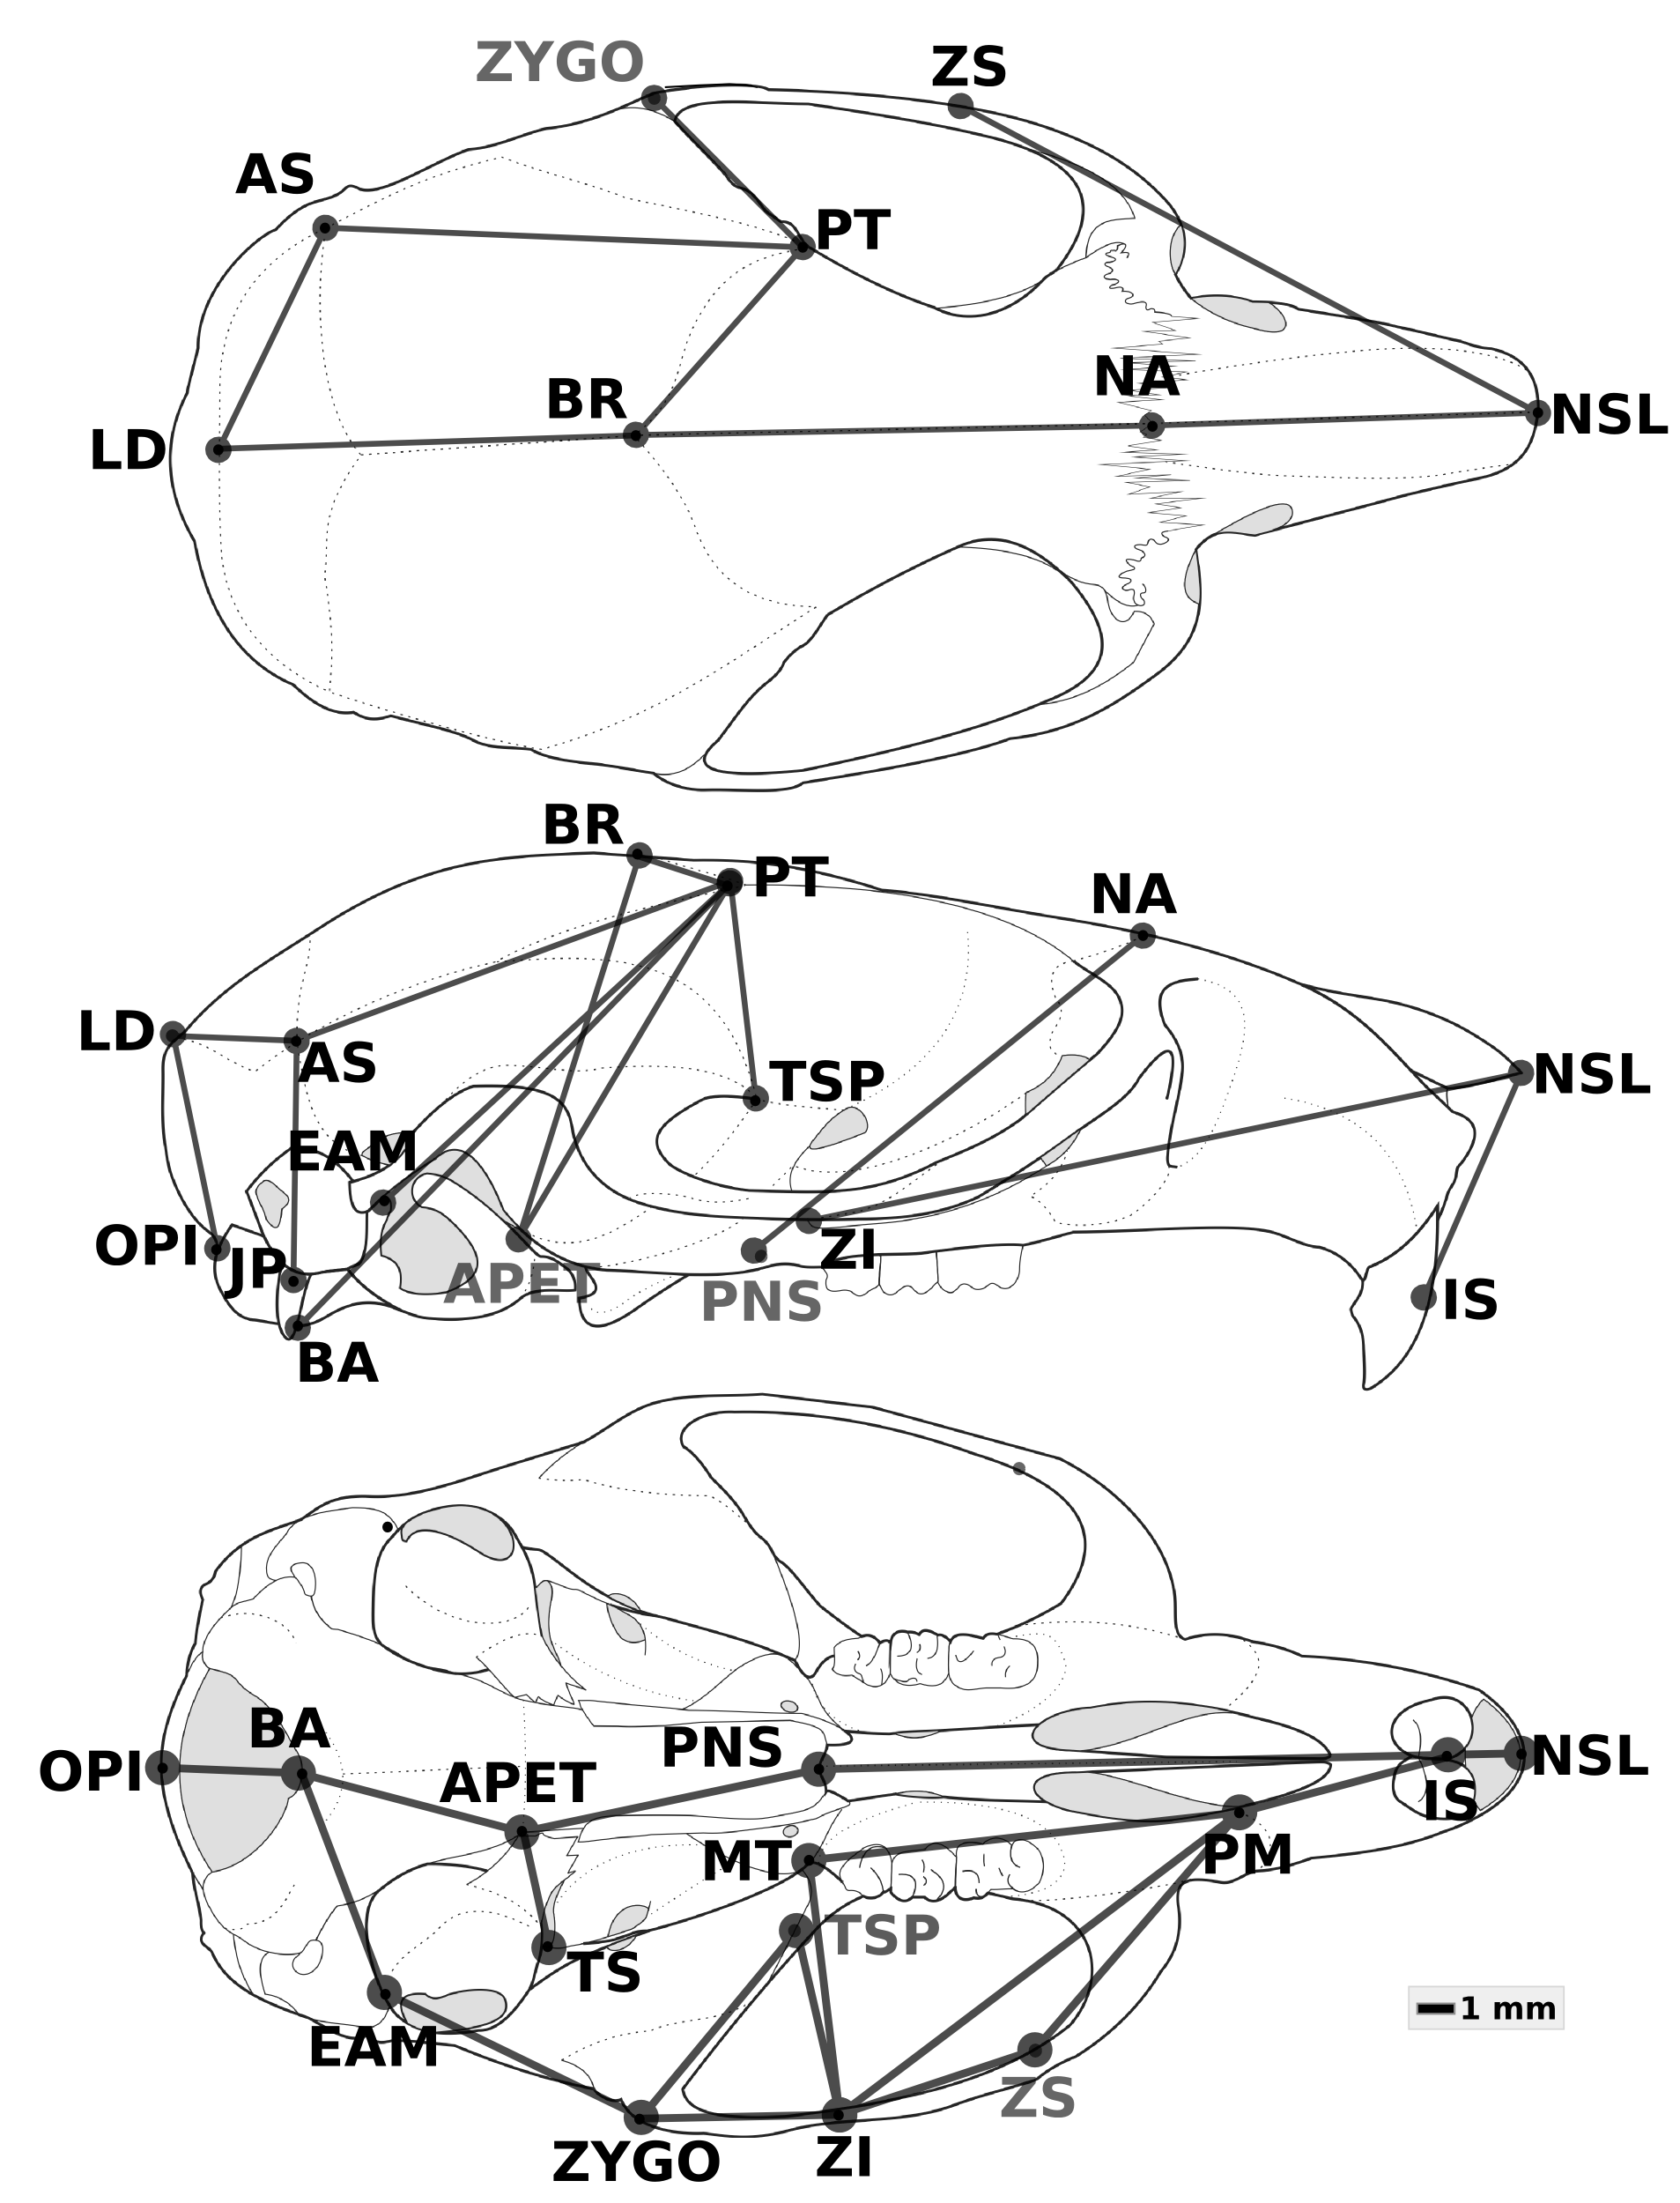
\includegraphics[width=\linewidth]{chapter_ratones/media/SI/figureS4.png}
    \caption[Cranial distances]{Cranial anatomical landmarks used in this study and
        set of euclidean distances calculated between them, following
    Cheverud (1995). Illustrations by Julia Laterza Barbosa.}
    \label{figsup:landmarks}
\end{figure}

\begin{figure}
    \centering
    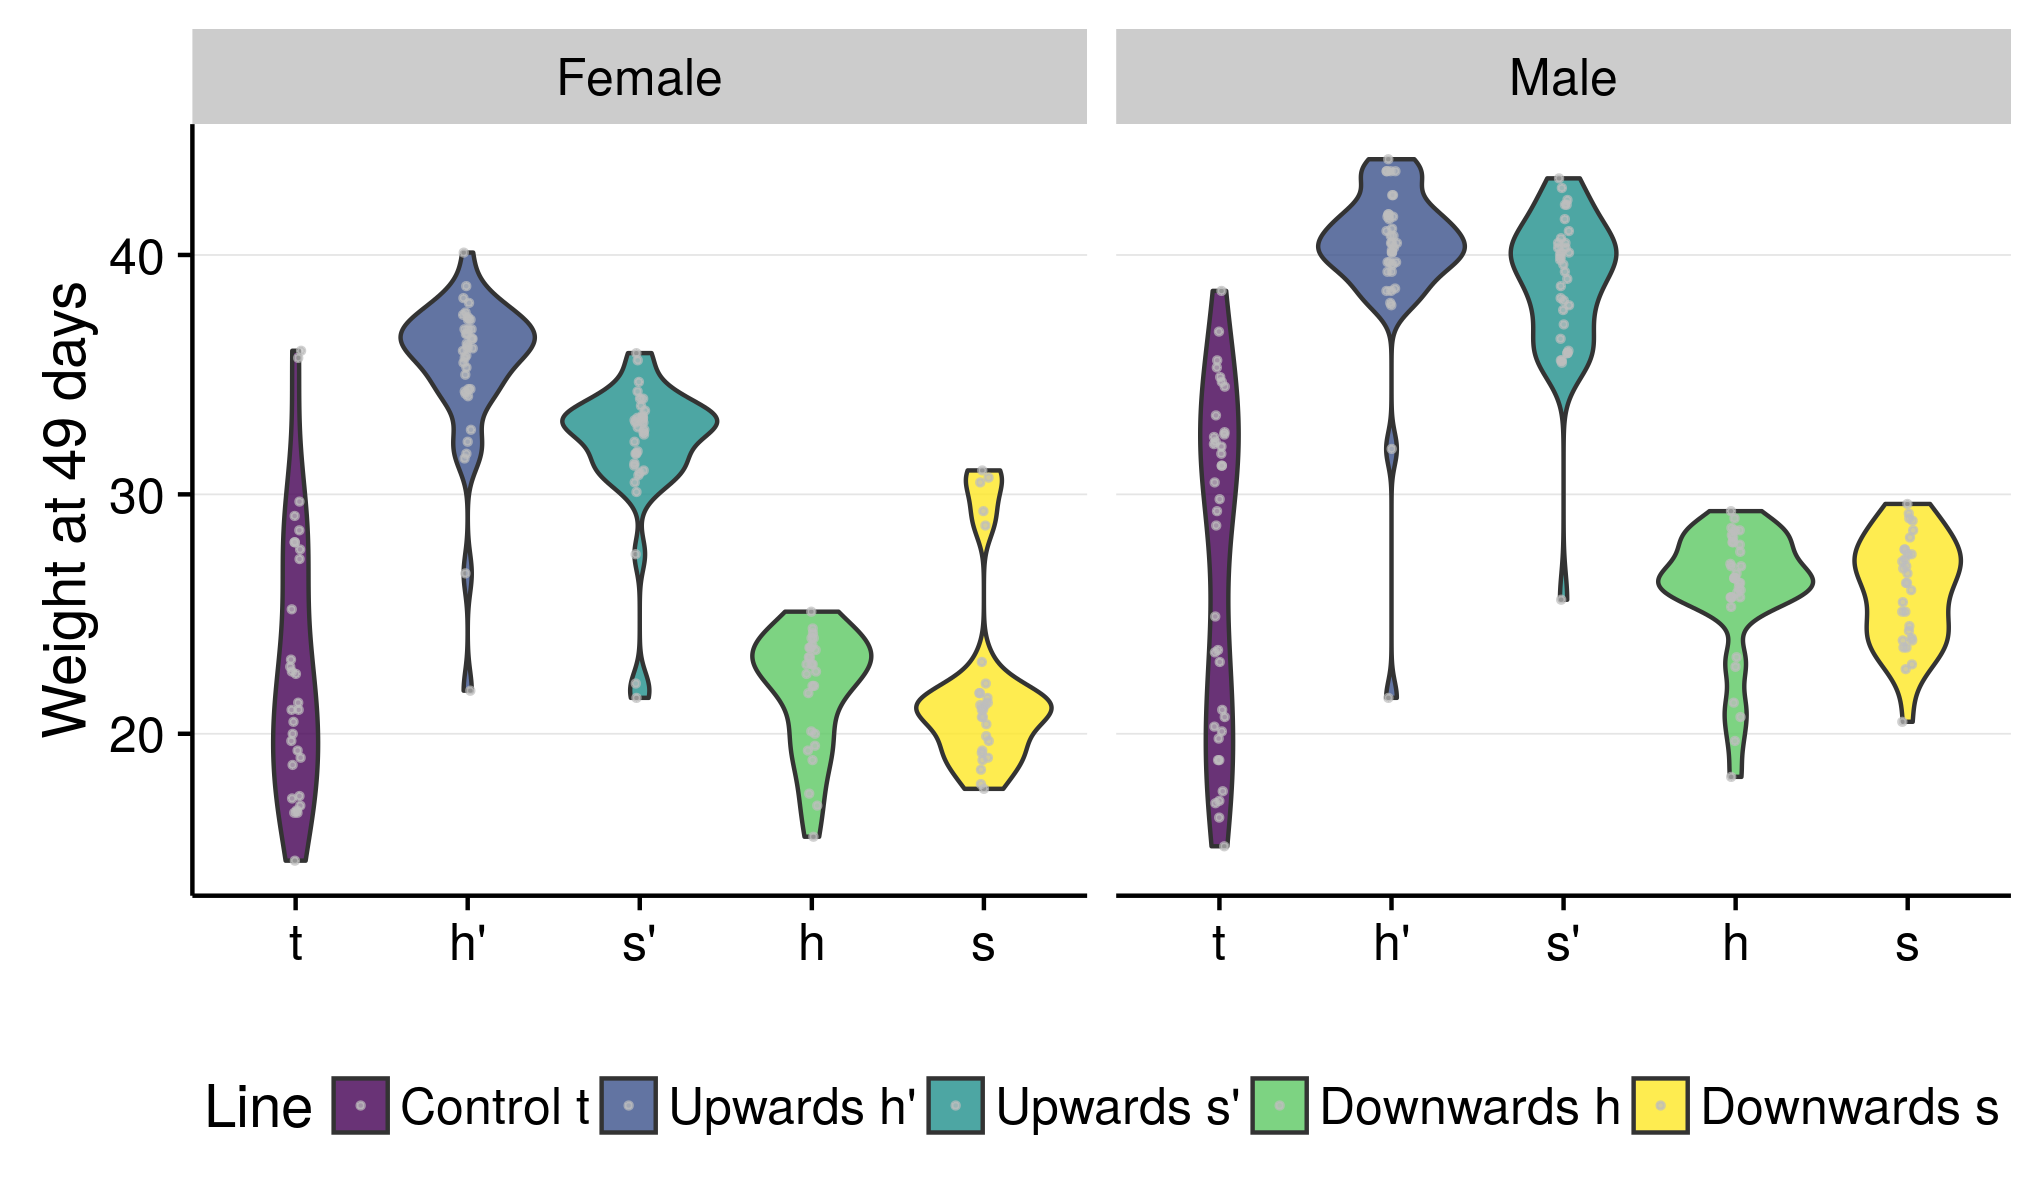
\includegraphics[width=15 cm]{chapter_ratones/media/SI/figureS5.png}
    \caption[Weight distribution per line]{Distribution of weight by line and sex. Selected lines
        have much lower variation, and upwards lines are larger than downwards
    lines, while control line has very large variance.}
    \label{figsup:weightchange}
\end{figure}

\begin{figure}
    \centering
    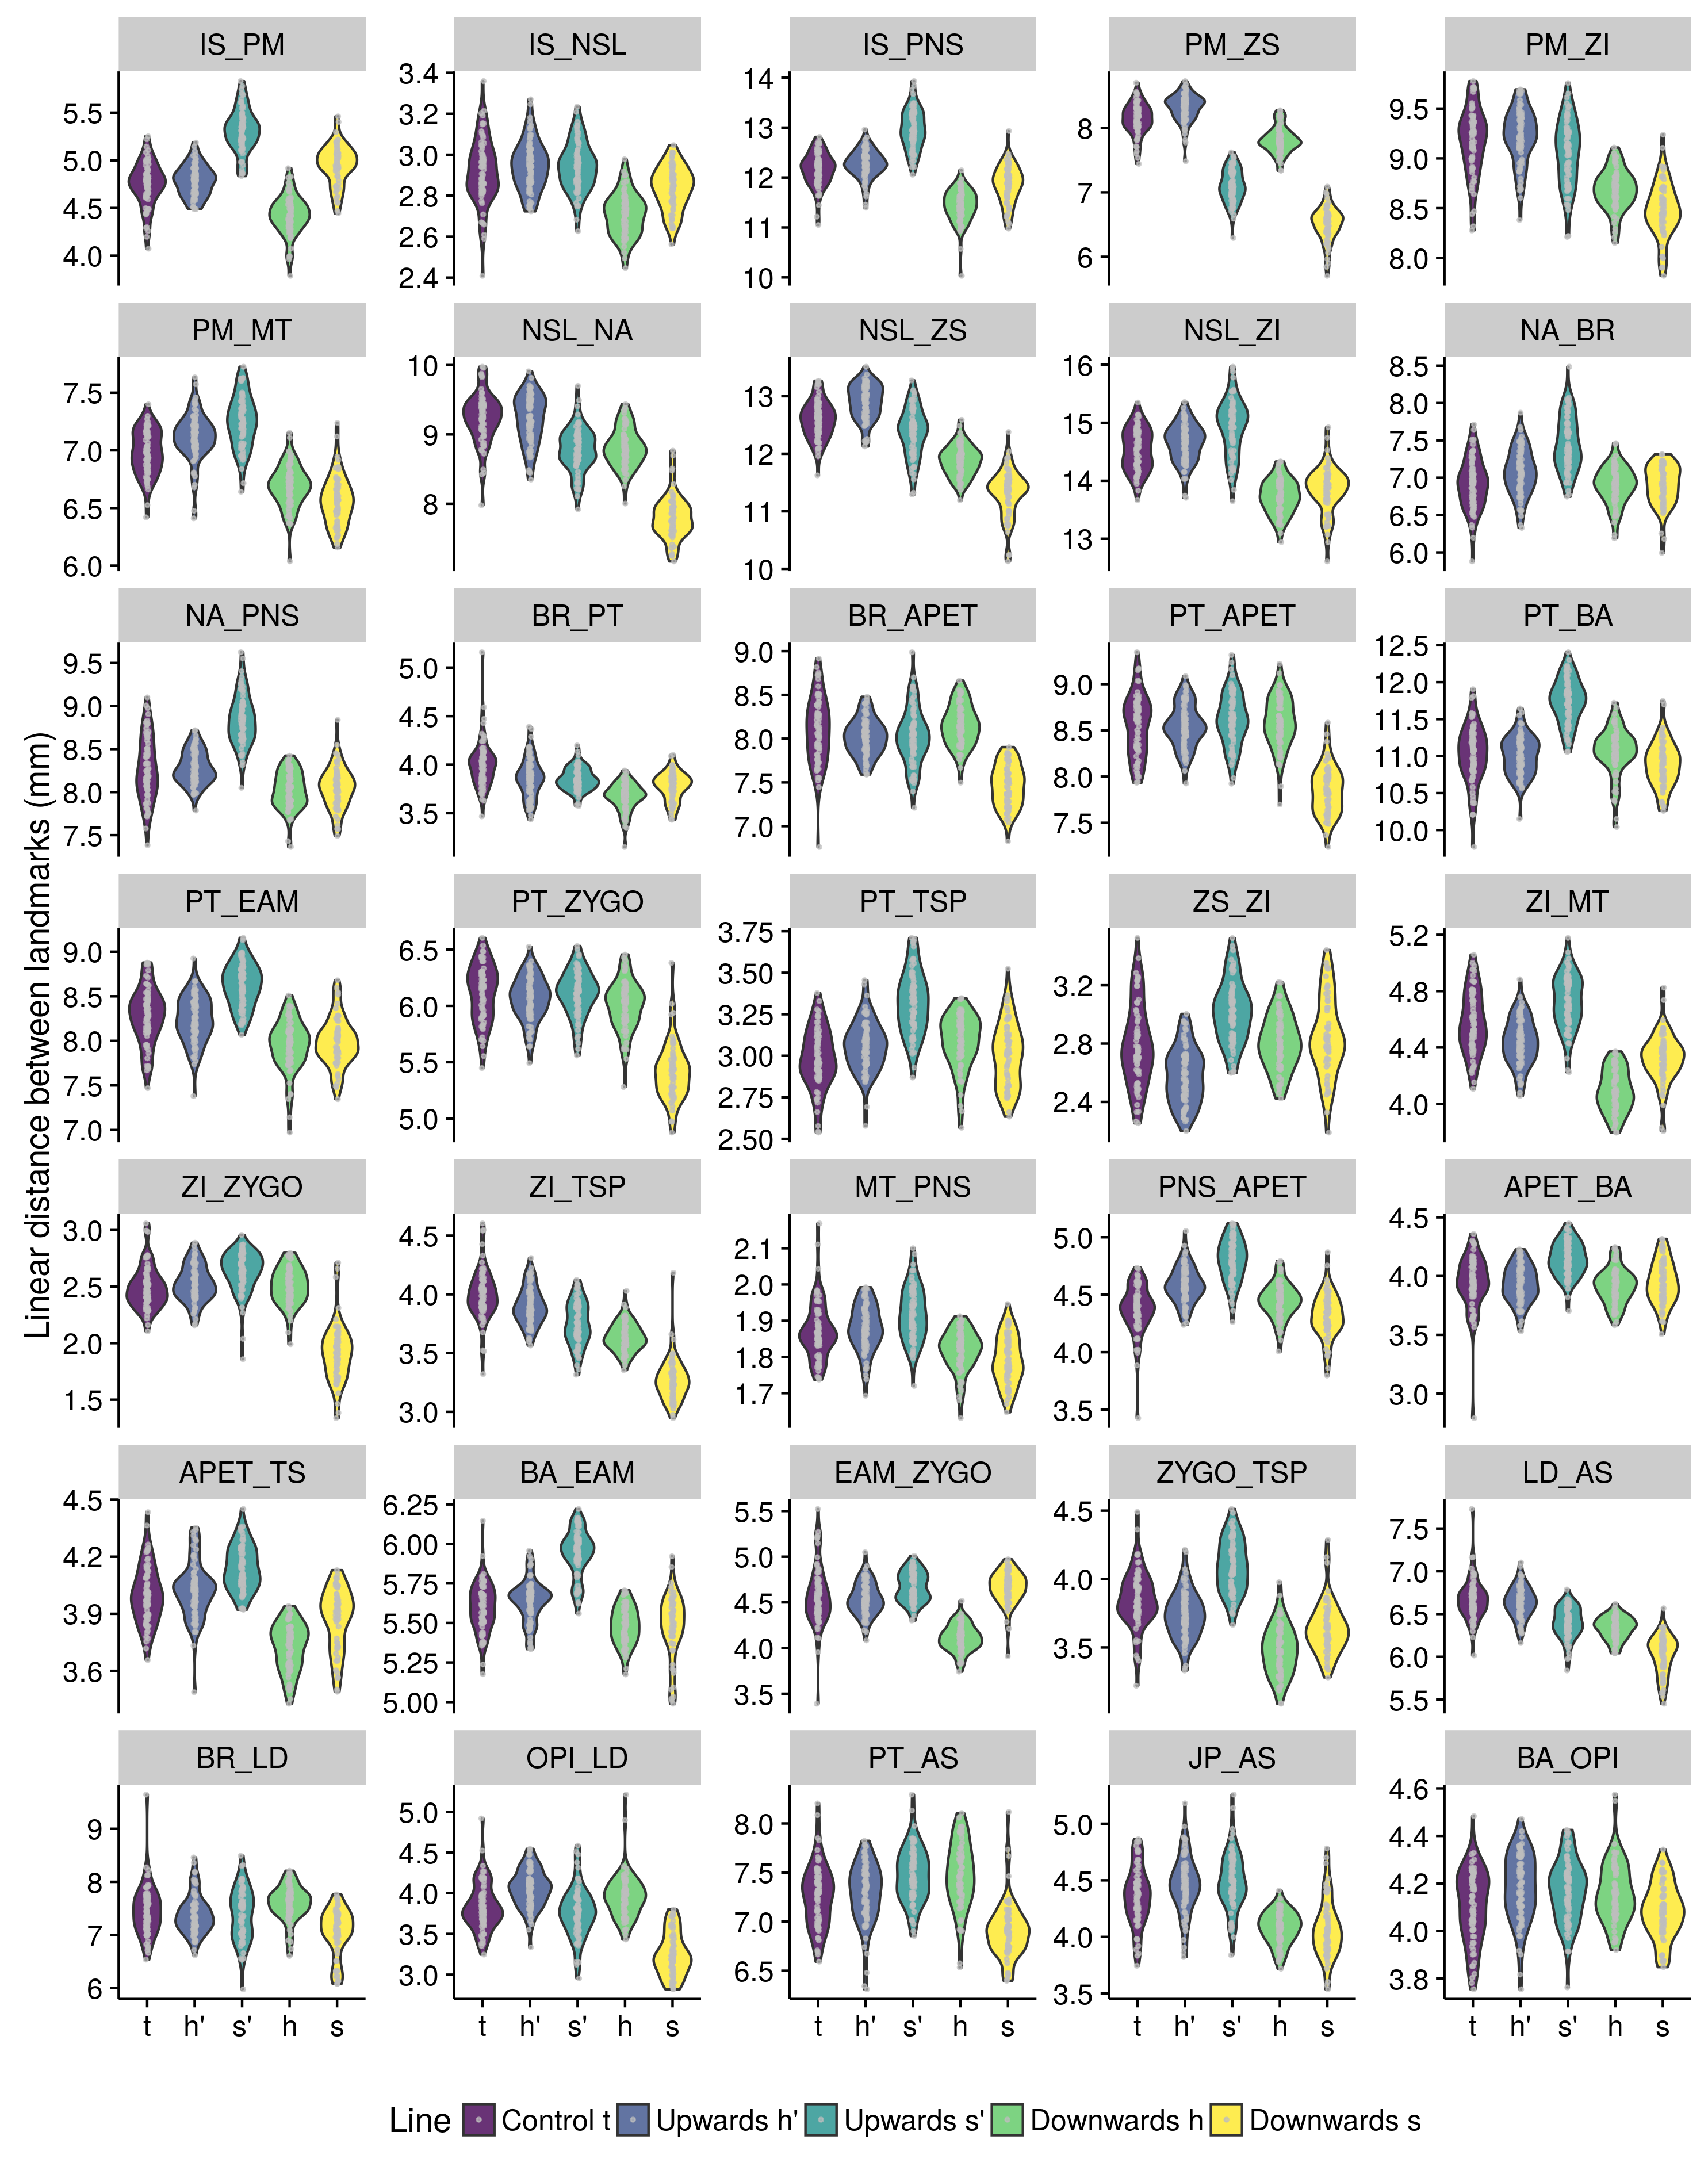
\includegraphics[width=\linewidth]{chapter_ratones/media/SI/figureS6.png}
    \caption[Distributions of cranial distances]{Distribution of all inter-landmark distances used in this
        study. In most cases, upwards lines are larger than downwards lines, but
        there are exceptions in the h line measurements, probably due to
        drift.}
    \label{figsup:traits}
\end{figure}

\begin{figure}
\centering
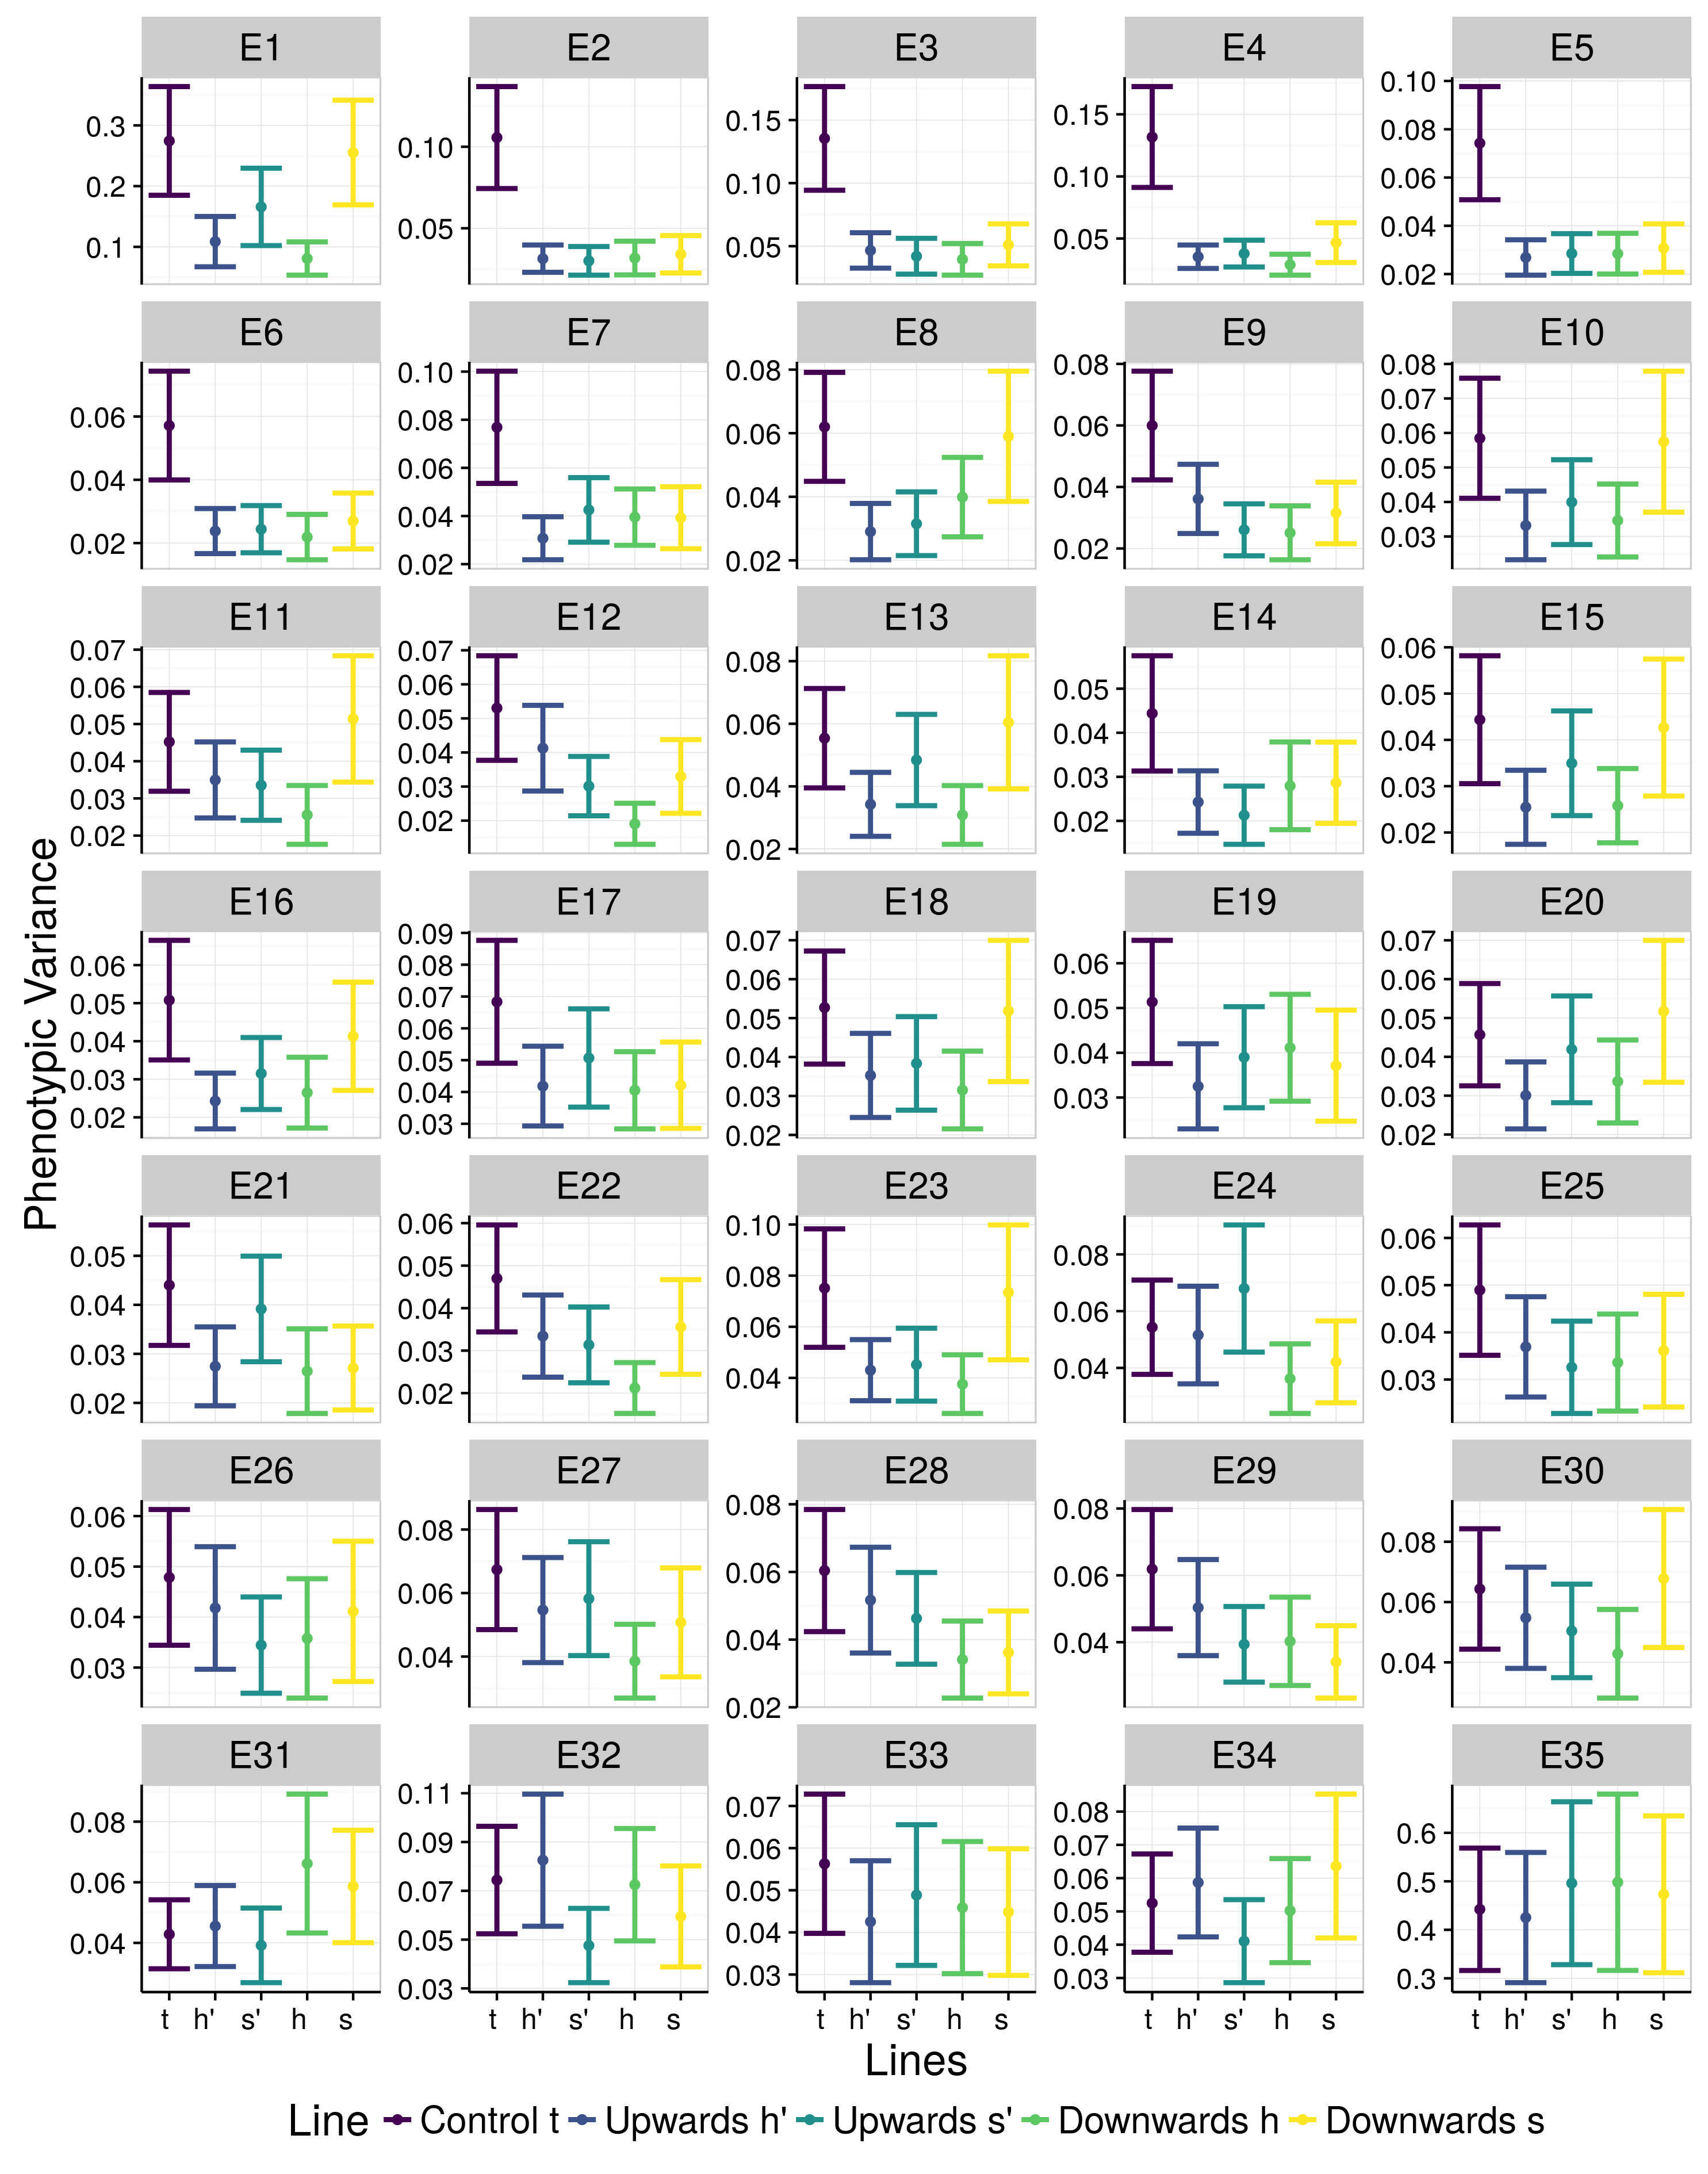
\includegraphics[width = \linewidth]{chapter_ratones/media/SI/figureS7.png}
\caption[Full matrix comparisons]{Bayesian Random Skewers results for all 35 dimensions.}
\end{figure}

\begin{table}
\centering
\caption[G-matrix comparisons]{Comparison between the posterior mean G-matrix and all posterior median P-matrices and within groups P-matrix.}
\begin{tabular}{rccc}
  \hline
 Selection& Line & Random Skewers & Krzanowski \\
  \hline
 Control & t & 0.84 & 0.80 \\
 Downwards & h & 0.85 & 0.77 \\
 Downwards & s & 0.83 & 0.76 \\
 Upwards & h' & 0.84 & 0.80 \\
 Upwards & s' & 0.88 & 0.78 \\
 \hline
 Within Groups P-matrix & all & 0.95 & 0.86 \\
   \hline
\end{tabular}
\end{table}

\begin{figure}
\centering
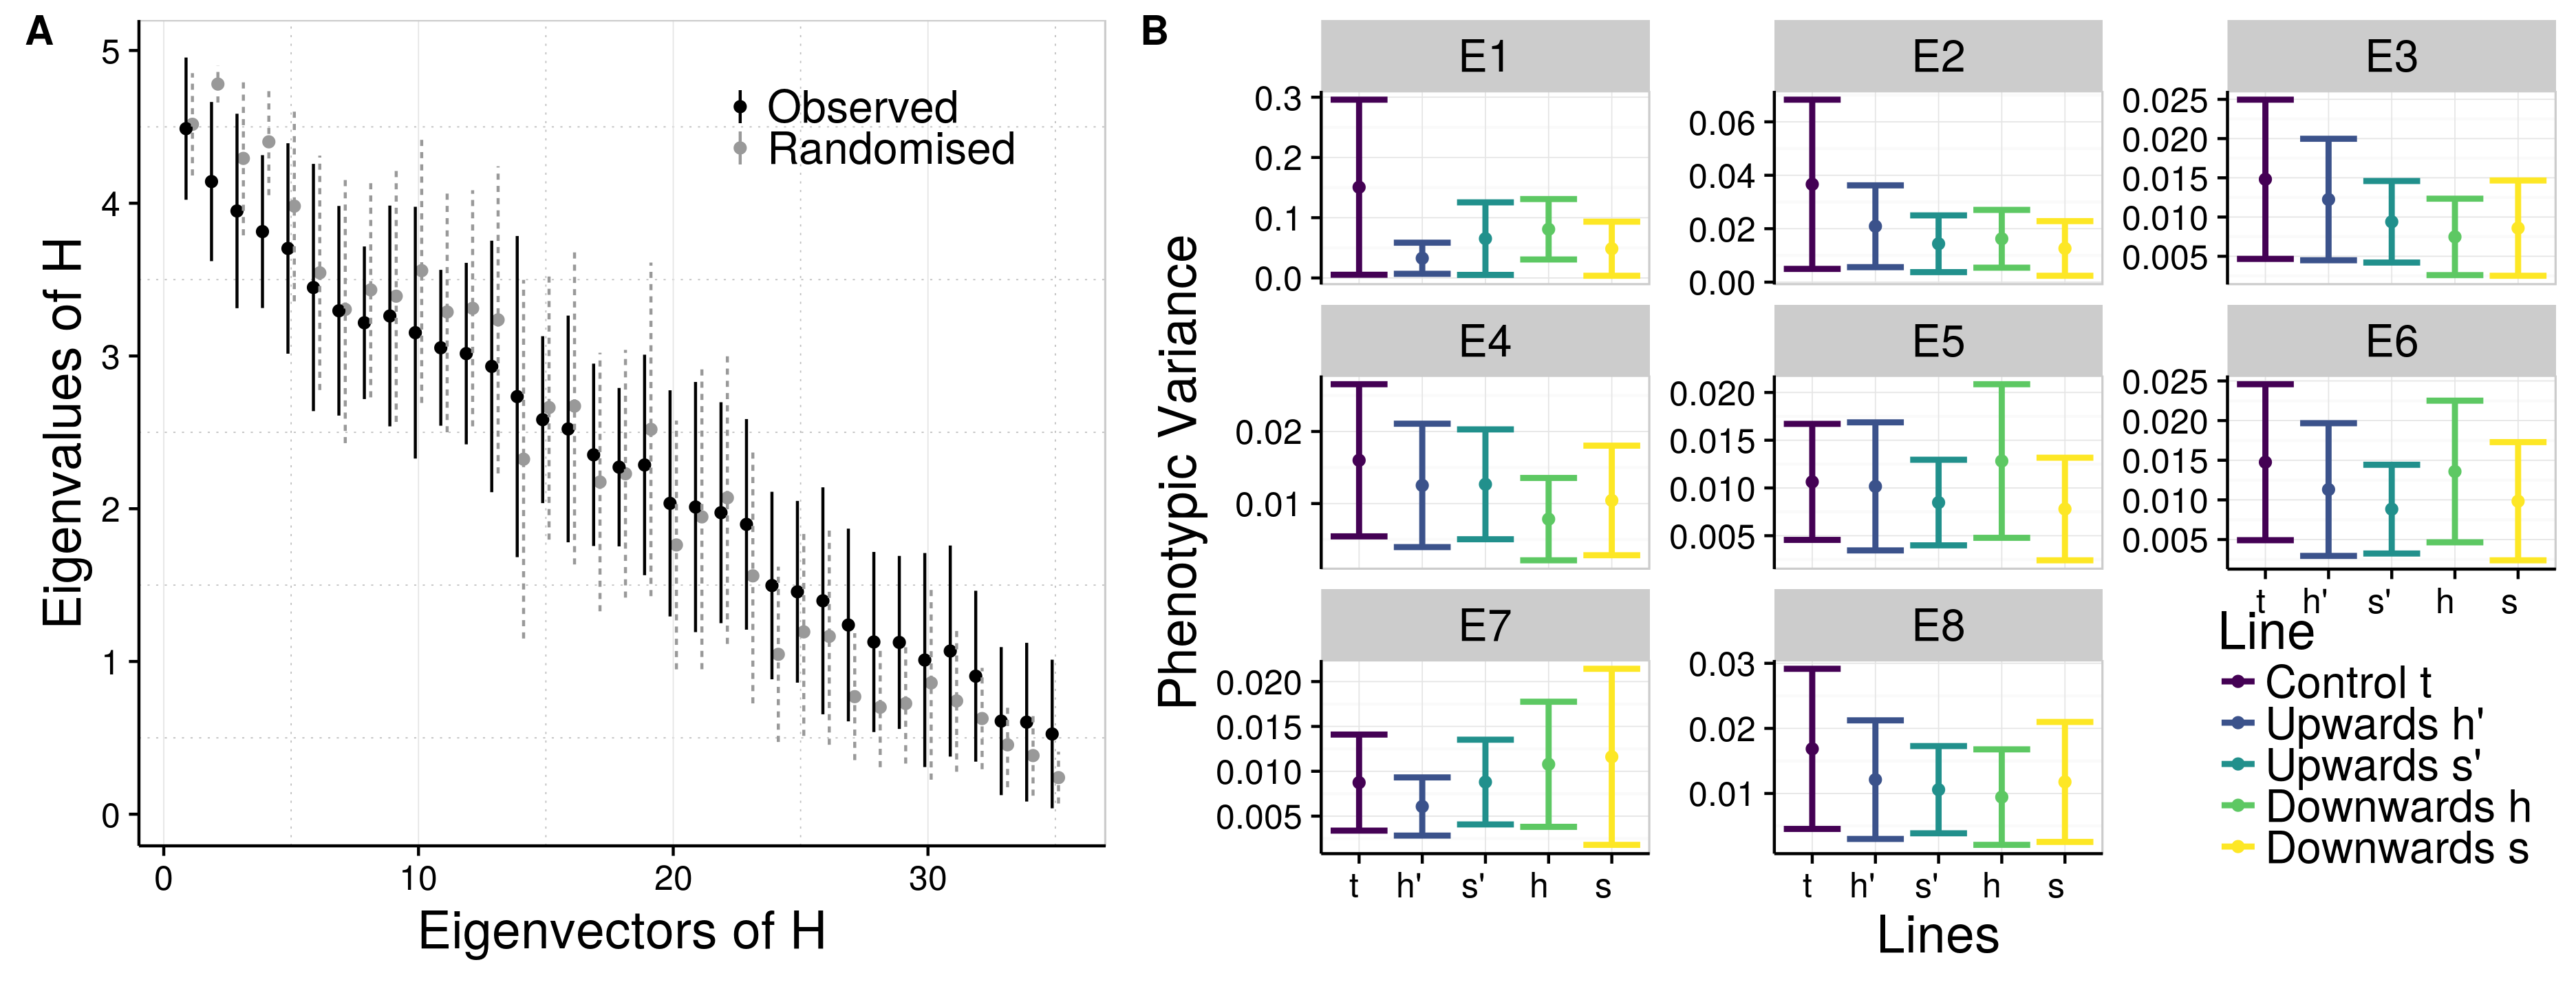
\includegraphics[width = \linewidth]{chapter_ratones/media/SI/figureS8_Fig2Gversion.png}
\caption[G matrix shared subspace]{(A) Krzanowski shared subspace; (B) Bayesian Random Skewers. Results obtained using the sample of G-matrices from the BSFG model.}
\end{figure}

\begin{table}
    \centering
    \caption[First eigenvectors per line]{First eigenvectors (E1) for the posterior median P-matrix for each line, and correlation of the E1s with an isometric size vector (a vector with equal loadings in all traits). Most loadings are positive or small,and correlation with isometric size vector is high (above 0.78) for all strains, indicating that all E1 are size related.}
    \begin{tabular}{rccccc}
        \hline
      & Control & Upwards  & Upwards & Downwards & Downwards  \\
                & t & h' &  s' &  h &  s \\

        \hline
  IS\_PM & 0.151 & -0.173 & -0.170 & -0.104 & 0.089 \\
  IS\_NSL & 0.007 & -0.020 & -0.029 & -0.033 & 0.020 \\
  IS\_PNS & 0.200 & -0.343 & -0.318 & -0.326 & 0.294 \\
  PM\_ZS & 0.110 & -0.093 & -0.145 & -0.201 & 0.209 \\
  PM\_ZI & 0.039 & -0.134 & -0.254 & -0.294 & 0.247 \\
  PM\_MT & 0.058 & -0.131 & -0.154 & -0.178 & 0.194 \\
  NSL\_NA & 0.087 & -0.191 & -0.112 & -0.226 & 0.155 \\
  NSL\_ZS & 0.091 & -0.172 & -0.346 & -0.336 & 0.318 \\
  NSL\_ZI & 0.160 & -0.246 & -0.419 & -0.396 & 0.350 \\
  NA\_BR & 0.055 & -0.065 & -0.142 & -0.258 & 0.156 \\
  NA\_PNS & 0.363 & -0.184 & -0.016 & -0.138 & 0.158 \\
  BR\_PT & -0.032 & -0.069 & -0.009 & -0.056 & 0.020 \\
  BR\_APET & 0.378 & -0.200 & -0.028 & -0.094 & 0.251 \\
  PT\_APET & 0.366 & -0.312 & -0.165 & -0.184 & 0.220 \\
  PT\_BA & 0.425 & -0.381 & -0.213 & -0.251 & 0.291 \\
  PT\_EAM & 0.272 & -0.325 & -0.144 & -0.248 & 0.194 \\
  PT\_ZYGO & 0.239 & -0.237 & -0.104 & -0.161 & 0.182 \\
  PT\_TSP & 0.113 & -0.121 & -0.011 & -0.063 & 0.080 \\
  ZS\_ZI & 0.224 & -0.091 & -0.014 & -0.018 & 0.026 \\
  ZI\_MT & 0.018 & -0.067 & -0.143 & -0.133 & 0.065 \\
  ZI\_ZYGO & -0.022 & -0.034 & -0.021 & -0.002 & 0.071 \\
  ZI\_TSP & 0.075 & -0.074 & -0.030 & -0.077 & 0.104 \\
  MT\_PNS & 0.024 & -0.037 & -0.003 & -0.024 & 0.034 \\
  PNS\_APET & 0.081 & -0.105 & -0.150 & -0.099 & 0.130 \\
  APET\_BA & 0.073 & -0.061 & -0.070 & -0.096 & 0.082 \\
  APET\_TS & 0.039 & -0.050 & -0.113 & -0.070 & 0.045 \\
  BA\_EAM & 0.058 & -0.080 & -0.176 & -0.084 & 0.094 \\
  EAM\_ZYGO & 0.087 & -0.091 & 0.015 & -0.087 & 0.039 \\
  ZYGO\_TSP & 0.044 & -0.112 & 0.003 & -0.092 & 0.107 \\
  LD\_AS & 0.021 & -0.050 & -0.226 & -0.055 & 0.079 \\
  BR\_LD & 0.067 & -0.195 & -0.382 & -0.025 & 0.192 \\
  OPI\_LD & 0.123 & -0.002 & 0.083 & -0.081 & 0.171 \\
  PT\_AS & 0.195 & -0.263 & -0.080 & -0.145 & 0.150 \\
  JP\_AS & 0.018 & -0.063 & -0.154 & -0.120 & 0.167 \\
  BA\_OPI & -0.007 & 0.030 & 0.008 & 0.000 & 0.026 \\
        \hline
        Correlation with \\ isometric vector & 0.71 & 0.80 &  0.72 &  0.85 & 0.85 \\
    \end{tabular}
\end{table}

\begin{table}
\centering
\caption[Matrix statistics confidence intervals]{95\% confidance interval and mean of the curves of posterior distributions obtained using the sample of P-matrices from the BSFG model from Figure 3.}
\begin{tabular}{rllccc}
  \hline
variable & selection & line & ic.min & mean & ic.max \\
  \hline
\textbf{A. Mean Squared Correlation} & control & t & 0.04 & 0.05 & 0.07 \\
   & upwards & h' & 0.06 & 0.07 & 0.10 \\
   & upwards & s' & 0.06 & 0.09 & 0.12 \\
   & downwards & h & 0.07 & 0.10 & 0.14 \\
   & downwards & s & 0.07 & 0.09 & 0.11 \\
\textbf{B. Proportion of Variation in E1} & control & t & 0.19 & 0.24 & 0.31 \\
   & upwards & h' & 0.23 & 0.30 & 0.37 \\
   & upwards & s' & 0.26 & 0.33 & 0.42 \\
   & downwards & h & 0.28 & 0.37 & 0.47 \\
   & downwards & s & 0.25 & 0.32 & 0.41 \\
\textbf{C. Mean Evolvability} & control & t & 0.07 & 0.08 & 0.09 \\
   & upwards & h' & 0.05 & 0.05 & 0.06 \\
   & upwards & s' & 0.05 & 0.06 & 0.07 \\
   & downwards & h & 0.04 & 0.05 & 0.06 \\
   & downwards & s & 0.05 & 0.06 & 0.07 \\
\textbf{D. Mean Flexibility} & control & t & 0.50 & 0.55 & 0.59 \\
   & upwards & h' & 0.47 & 0.51 & 0.56 \\
   & upwards & s' & 0.43 & 0.48 & 0.53 \\
   & downwards & h & 0.41 & 0.47 & 0.52 \\
   & downwards & s & 0.42 & 0.47 & 0.52 \\
  

   \hline
\end{tabular}
\end{table}

\begin{figure}
\centering
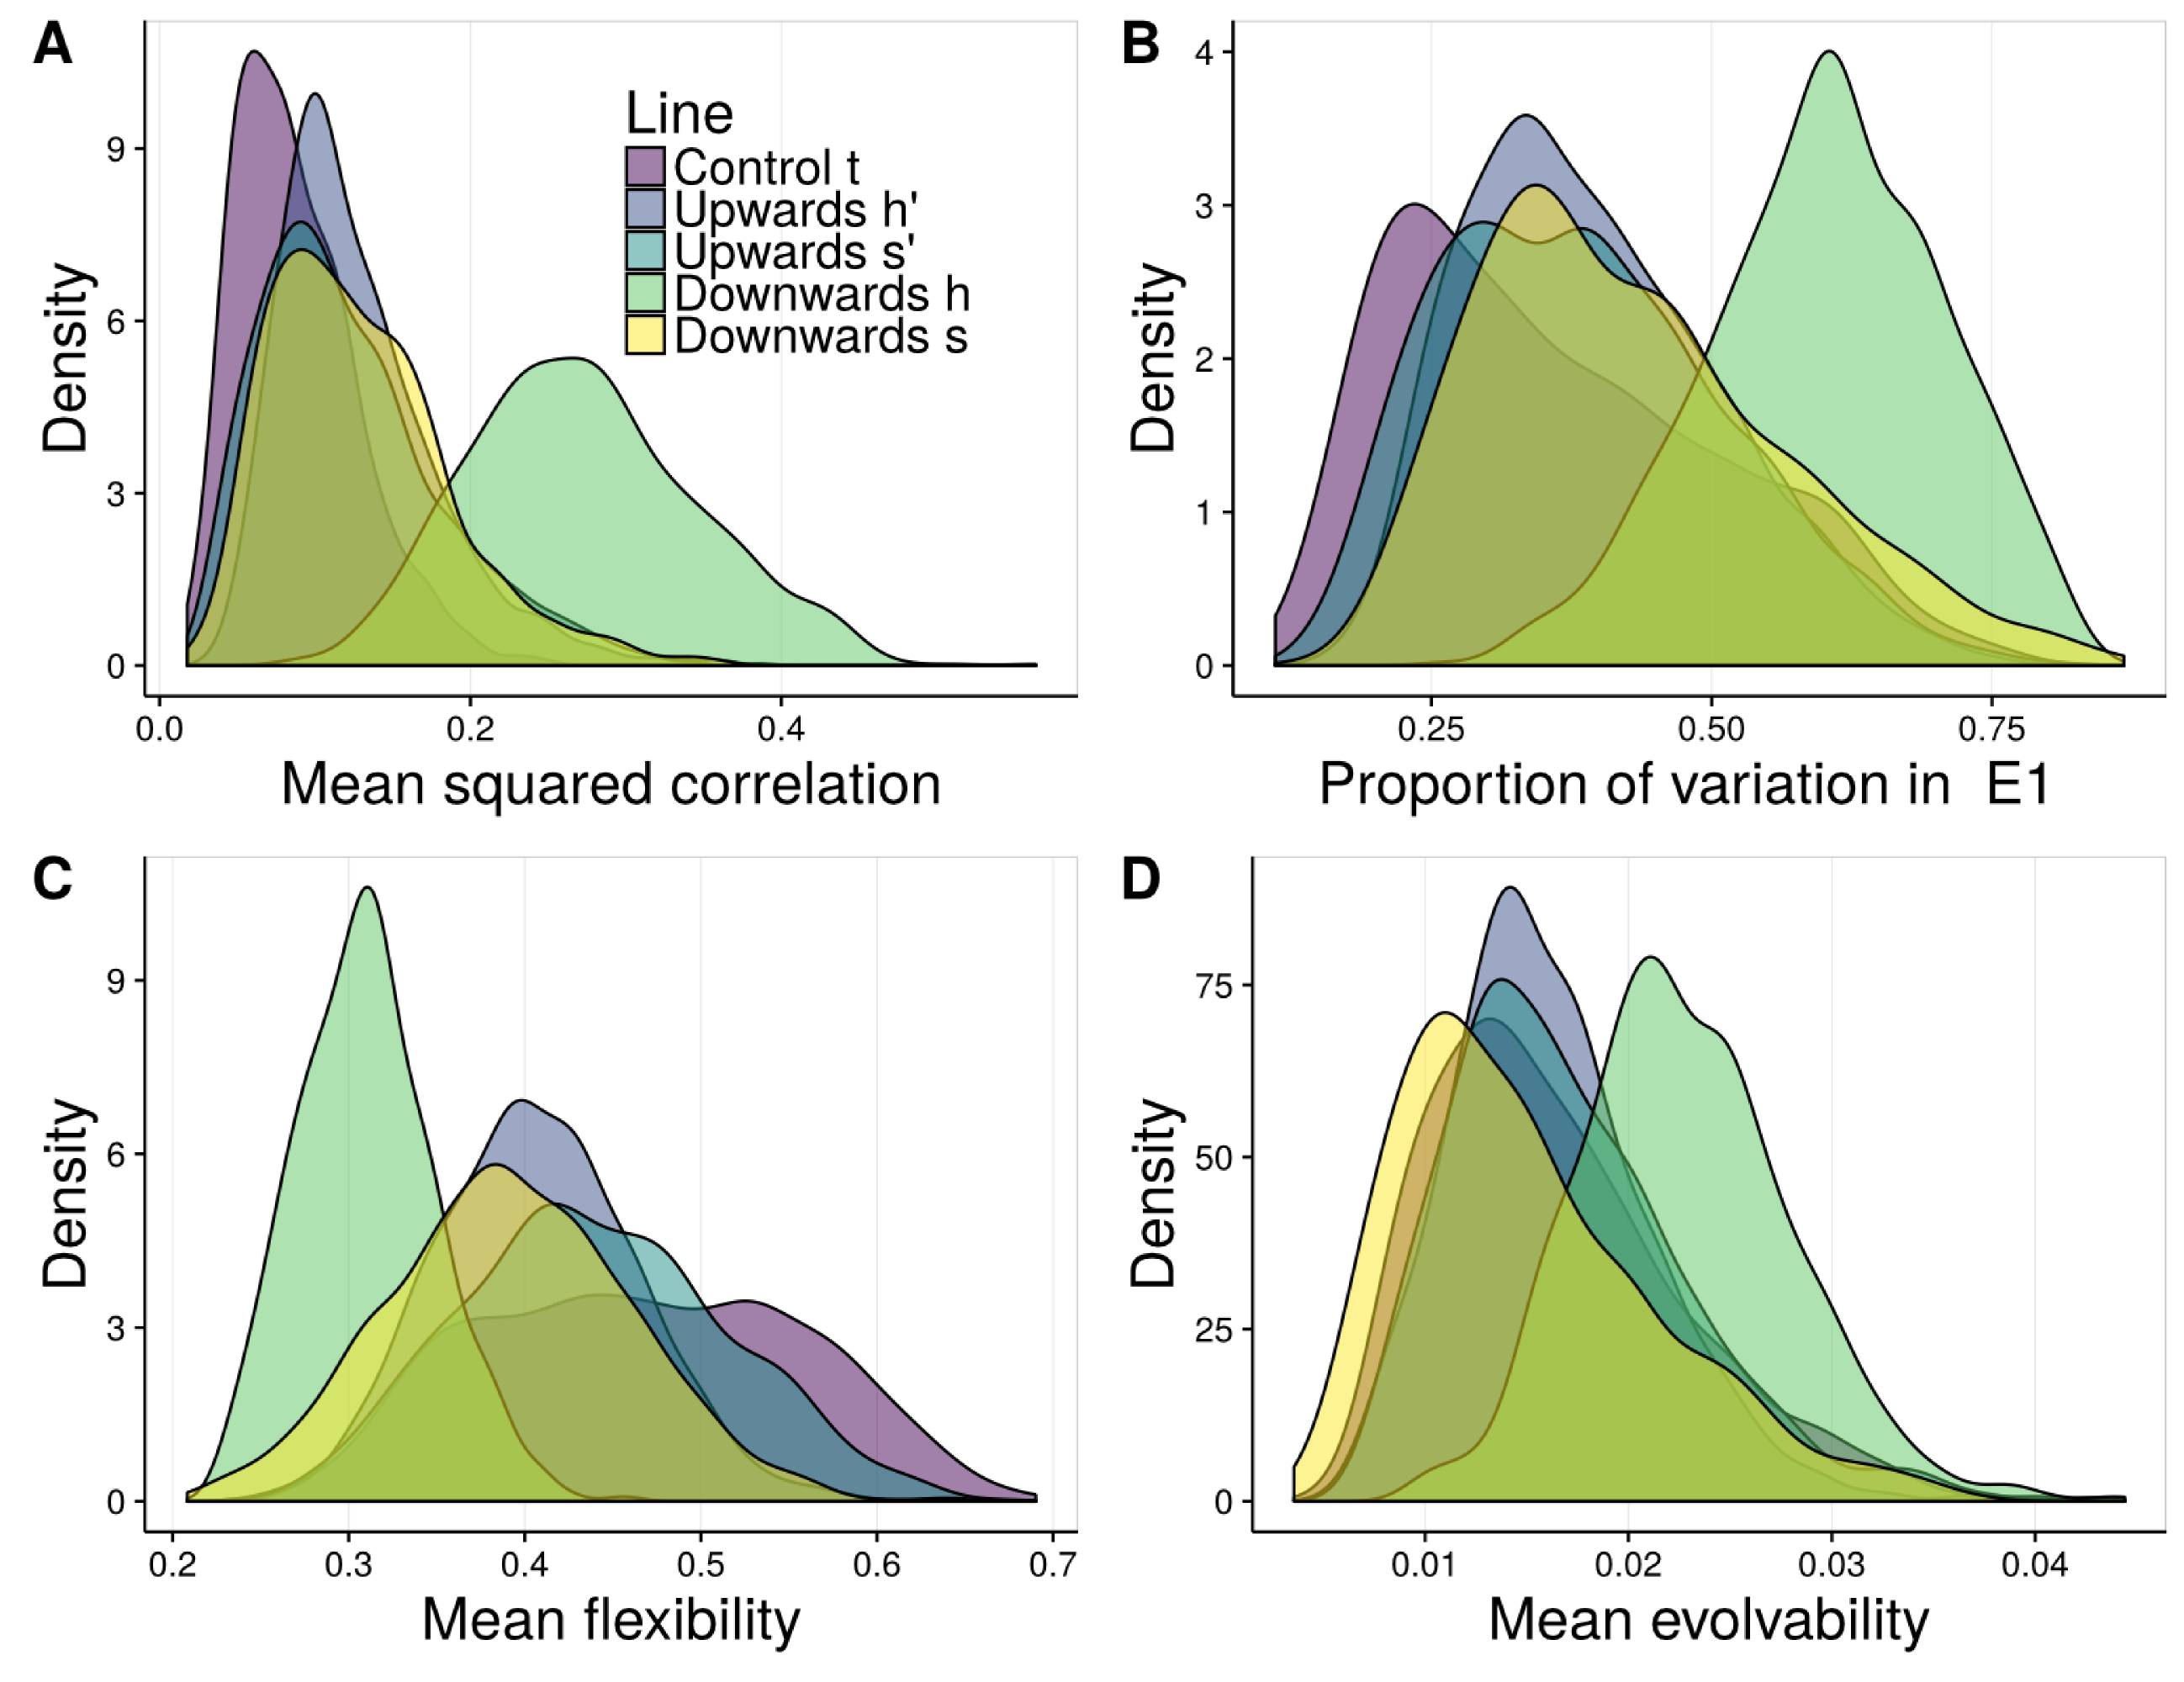
\includegraphics[width = 12cm]{chapter_ratones/media/SI/figureS9_Fig3Gversion.png}
\caption[G-matrix evolutionary statistics]{Comparison of covariation patterns between control and selected lines using evolutionary statistics (A) Overall integration measured as mean square correlation between all traits; (B) Proportion of variation associated with the first eigenvector, which is related to size variation; (C) Mean flexibility; (D) Mean evolvability. Curves represent posterior distributions obtained using the sample of G-matrices from the BSFG model.}
\end{figure}

\begin{table}
\centering
\caption[Directional matrix statistics confidence intervals]{95\% confidance interval and mean of the curves of posterior distributions obtained using the sample of P-matrices from the BSFG model from Figure 4.}
\begin{tabular}{rllccc}
  \hline
variable & selection & line & ic.min & mean & ic.max \\
  \hline
\textbf{A. Scaled directional evolvability} & control & t & 4.10 & 5.26 & 6.73 \\
  & downwards & h & 6.74 & 8.92 & 11.59 \\
   & downwards & s & 6.58 & 8.36 & 10.64 \\
   & upwards & h' & 7.04 & 9.11 & 11.48 \\
   & upwards & s' & 7.37 & 9.68 & 12.43 \\
\textbf{B. Scaled directional conditional evolvability} & control & t & 0.01 & 0.01 & 0.01 \\
   & downwards & h & 0.01 & 0.01 & 0.01 \\
   & downwards & s & 0.01 & 0.01 & 0.02 \\
   & upwards & h' & 0.01 & 0.02 & 0.02 \\
   & upwards & s' & 0.01 & 0.01 & 0.02 \\
\textbf{C. Vector correlation with E1} & control & t & 0.30 & 0.61 & 0.84 \\
   & downwards & h & 0.69 & 0.79 & 0.86 \\
   & downwards & s & 0.56 & 0.80 & 0.91 \\
   & upwards & h' & 0.87 & 0.92 & 0.96 \\
   & upwards & s' & 0.76 & 0.89 & 0.94 \\
   \hline
\end{tabular}
\end{table}

\begin{figure}
\centering
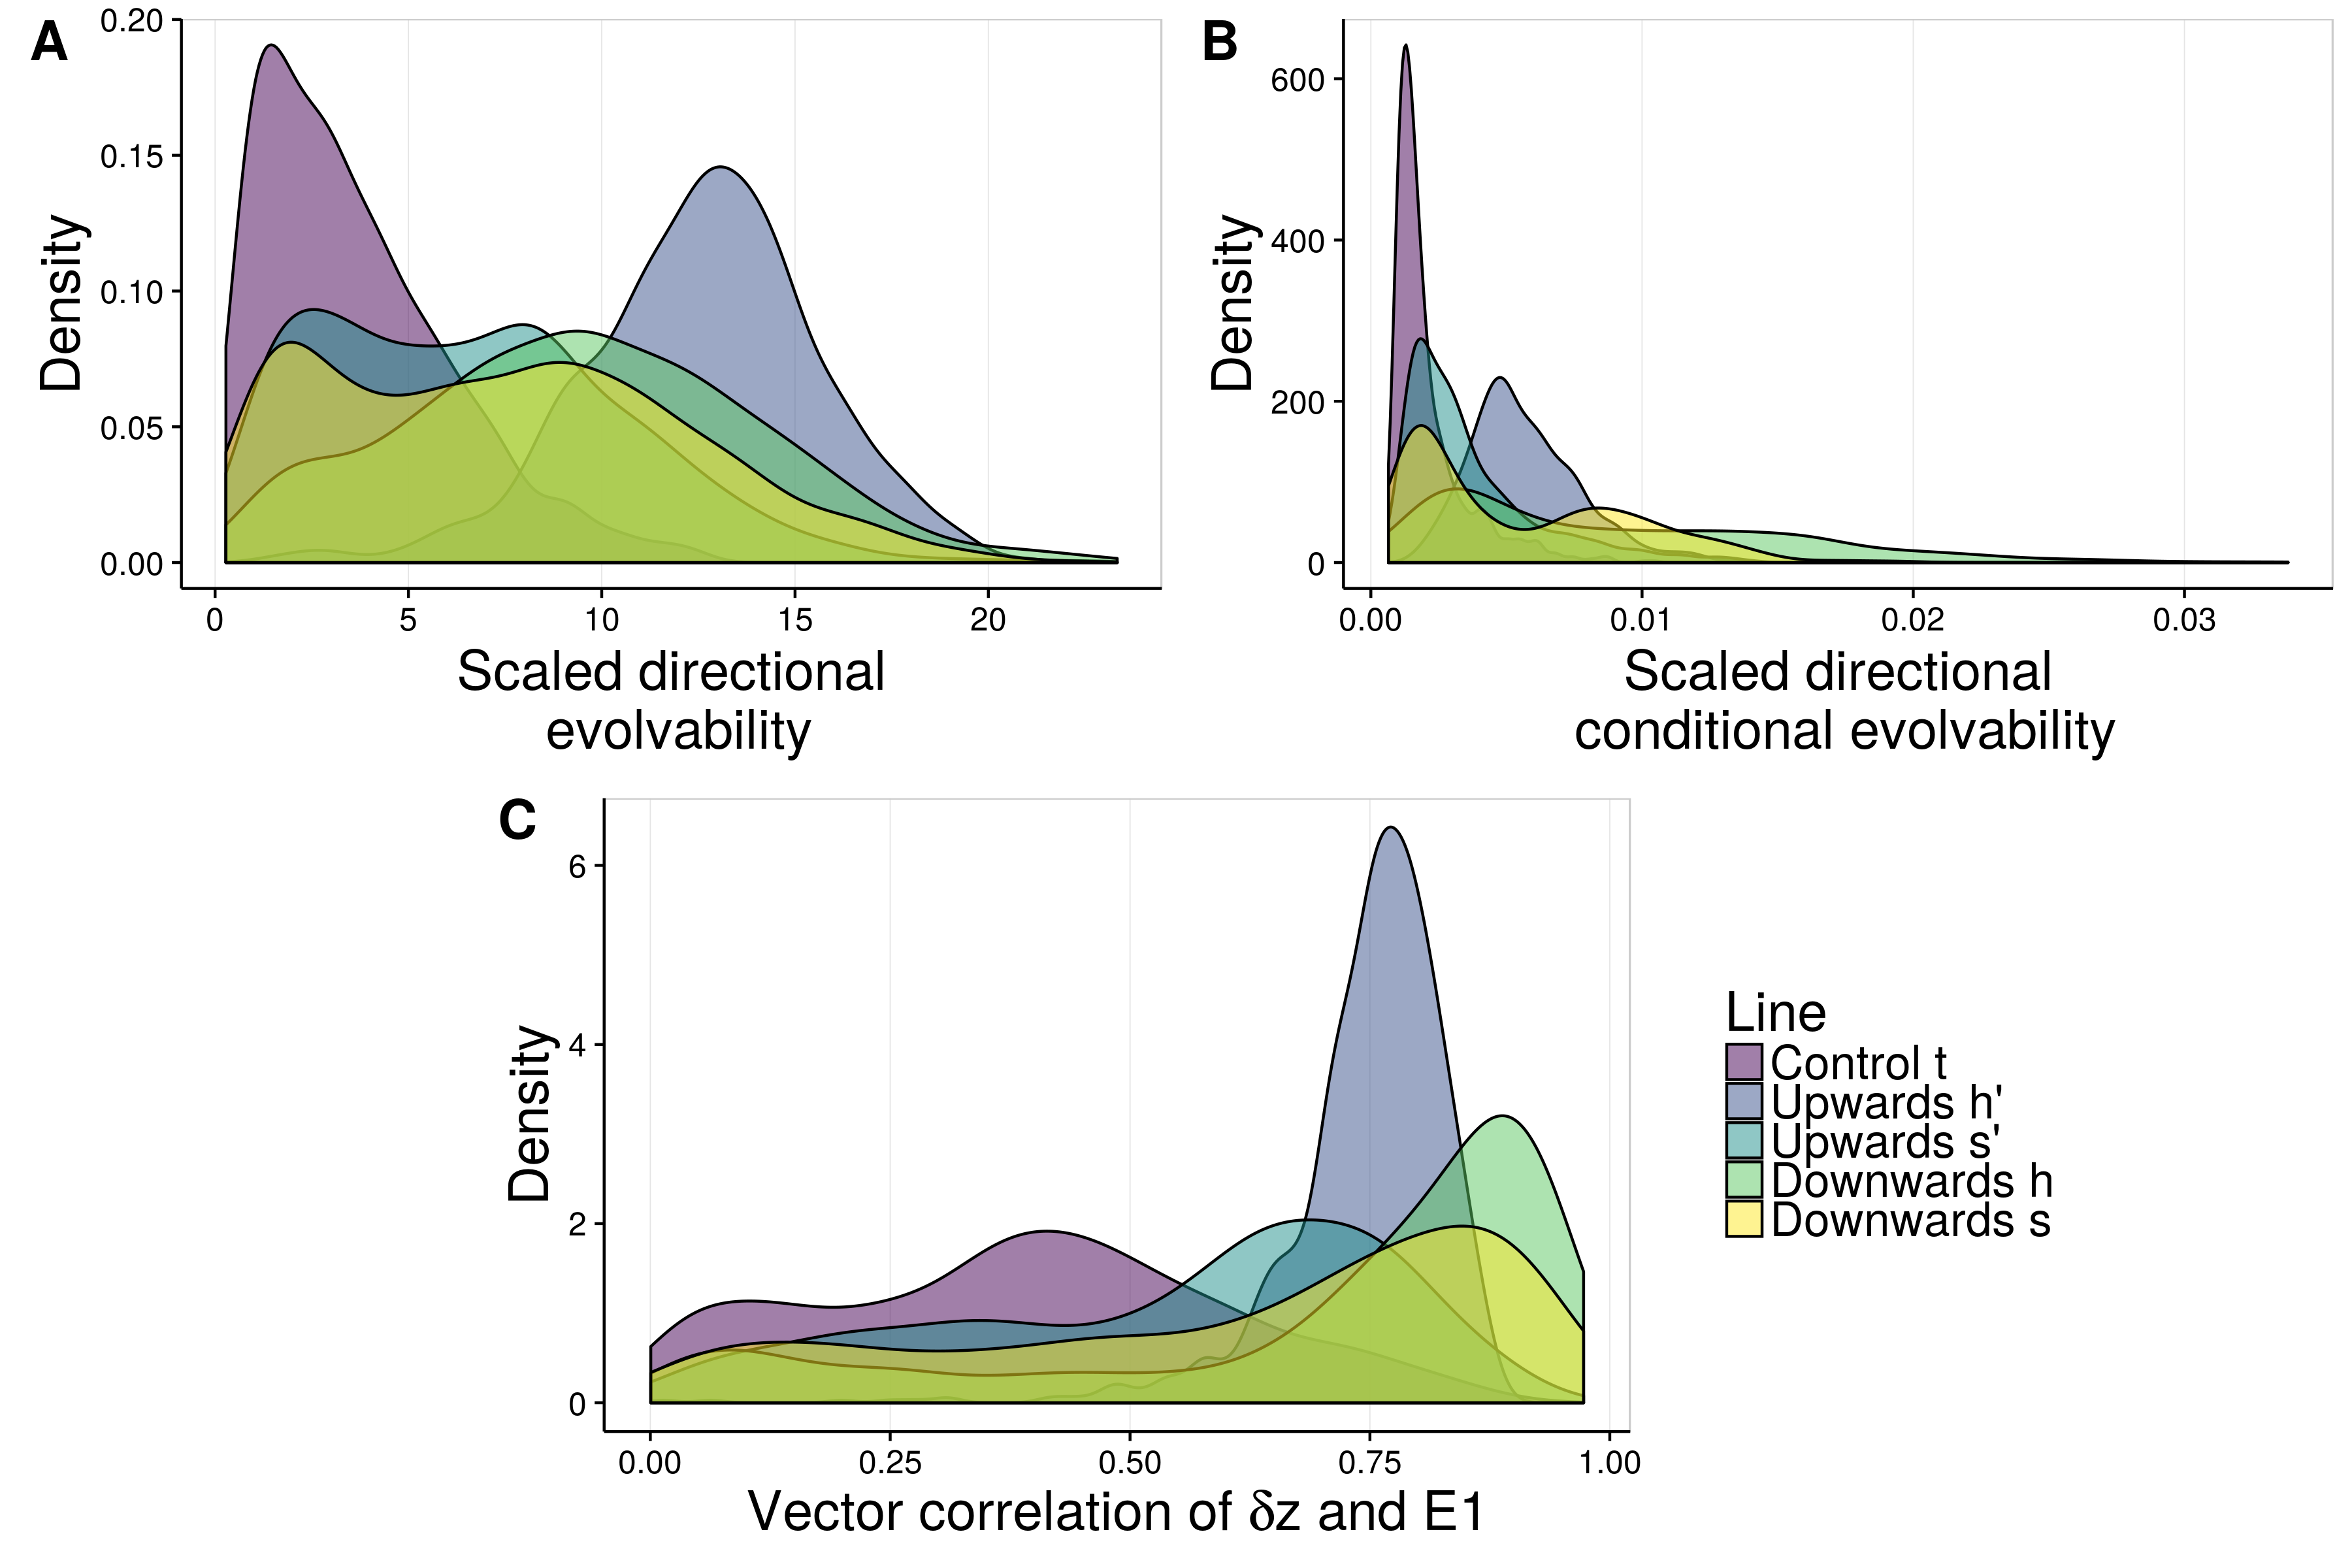
\includegraphics[width = 12cm]{chapter_ratones/media/SI/figureS10_Fig4Gversion.png}
\caption[Directional evolutionary statistics in the G-matrix]{(A) Scaled direction evolvability, the ratio of evolvability in the direction of $\delta z$ and the mean evolvability for each line; (B) Scaled direction conditional evolvability, the ratio of conditional evolvability in the direction of $\delta z$ and the mean conditional evolvability for each line; (C) the vector correlation between $\delta z$ and first eigenvector for each line. Curves represent posterior distributions obtained using the sample of G-matrices from the BSFG model.}
\end{figure}
% section supporting_information (end)

\end{refsection}
